\documentclass[10pt]{beamer}
\usepackage{lmodern}
%\usetheme{Darmstadt}
\usetheme{Frankfurt}
\usepackage{tcolorbox}
%\usepackage{beamerthemesplit}
\usepackage{appendixnumberbeamer}
\usefonttheme{serif}
\useinnertheme{circles}
\setbeamertemplate{footline}[page number]{}
\setbeamertemplate{navigation symbols}{}
\setbeamercolor{block title}{bg=blue!30,fg=black}
%\usepackage[timeinterval=10,timeduration=2.0]{tdclock}
\usepackage{tikz}
\usepackage{graphicx}
\usepackage{subfig}
\usepackage{latexsym,amsmath,amssymb}
\usepackage{multirow}
\usepackage{amsthm}
\usepackage{epstopdf}
\usepackage{booktabs}
\usepackage{mathrsfs}
\usepackage{boldline}
\usepackage{tabularx}
\usepackage{stackengine}
\usetikzlibrary{arrows,shapes,calc}

%\usepackage[inline]{enumitem}
\usepackage{caption}
%\usepackage{subcaption}
\newcommand{\R}{{\mathbb R}}
\newcommand{\C}{{\mathbb C}}
\newcommand{\sign}{\mathop{\bf sign}}
\newcommand{\N}{\mathcal{N}}
\newcommand{\argmin}{\mathop{\rm argmin}}
\newcommand{\etc}{{\it etc.}}
\newcommand{\eg}{{\it e.g.}}
\newtheorem{proposition}[theorem]{Proposition}

\usepackage{listings}
%From CI paper
\let\oldcite=\cite                                                              
\renewcommand{\cite}[1]{\textcolor[rgb]{0.2,0.5,.3}{\oldcite{#1}}}
\definecolor{mycite}{rgb}{0.4,0.0,0.8}
\definecolor{myhighlight1}{rgb}{0.758, 0.2, 0.078}
\definecolor{mycite2}{rgb}{0.2,0.5,.3}


\newcommand\blfootnote[1]{%
  \begingroup
  \renewcommand\thefootnote{}\footnote{#1}%
  \addtocounter{footnote}{-1}%
  \endgroup
}
\graphicspath{ {Img/} }
\AtBeginSection[]{
	\begin{frame}{Outline}
		\tableofcontents[currentsection]
	\end{frame}
	}
\title[Deep Learning]{Introduction to Deep Learning in Vision: Basics, Optimization,  Networks and Coding}
\author[Yue Zhang]{Yue Zhang}
\institute[CWRU] {\footnotesize{Department of Mathematics, Applied Mathematics and Statistics\\ Case Western Reserve University}\\~ \\ \date \\}

\begin{document}

\begin{frame}
\titlepage
%\initclock
\end{frame}


\section{Overview}
\begin{frame}
\frametitle{Overview of the Journey}
	\begin{figure}[H]
		\centerline{
			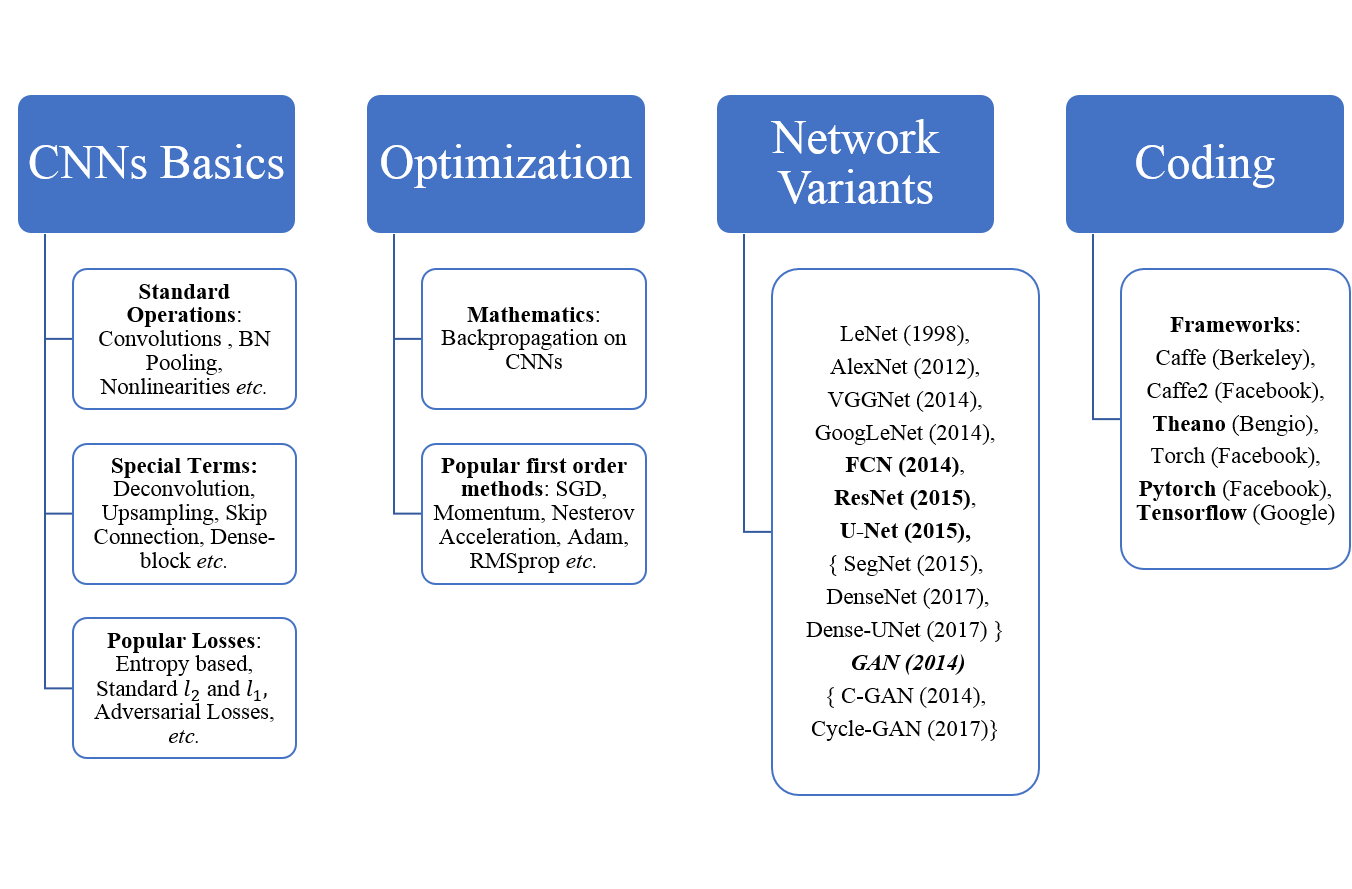
\includegraphics[width=1.1\textwidth]{overview.png}
		}
	\end{figure}
\end{frame}


\section{Convolutional Neural Networks Basics}
\subsection{Basic Operations}
\begin{frame}
	\frametitle{Basic Operations in  CNNs}
	Standard operations in a Convolutional Neural Network:
	\begin{itemize}
		\item Convolution
		\item Pooling 
		\item Batch Normalization
		\item Nonlinear Activation
		\item Others: Deconvolution, Upsampling,  Skip Connections \etc
	\end{itemize}
\end{frame}

\begin{frame}
	\frametitle{A Quick Example: UNet \blfootnote{\textcolor{mycite2}{Olaf Ronneberger, Philipp Fischer, Thomas Brox}.\textit{ U-Net: Convolutional Networks for Biomedical
			Image Segmentation}, MICCAI 2015.}}
	One of the most popular networks in semantic segmentation.
	\begin{figure}[H]
	\centerline{
		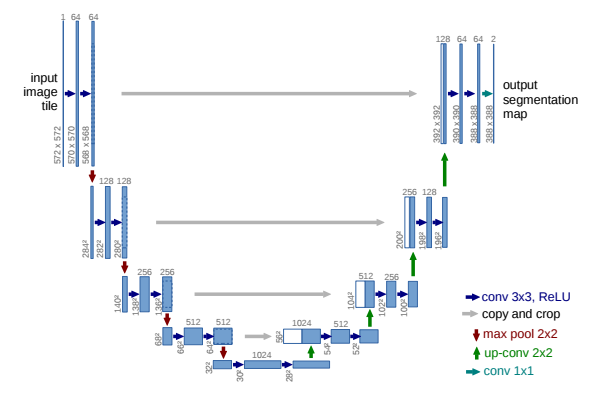
\includegraphics[width=0.8\textwidth]{unet.png}
	}
	\end{figure}
\end{frame}

\begin{frame}
	\frametitle{A Quick Example: UNet \blfootnote{\textcolor{mycite2}{Olaf Ronneberger, Philipp Fischer, Thomas Brox}.\textit{ U-Net: Convolutional Networks for Biomedical
			Image Segmentation}, MICCAI 2015.}}
		One of the most popular networks in semantic segmentation.
	\begin{figure}[H]
		\centerline{
			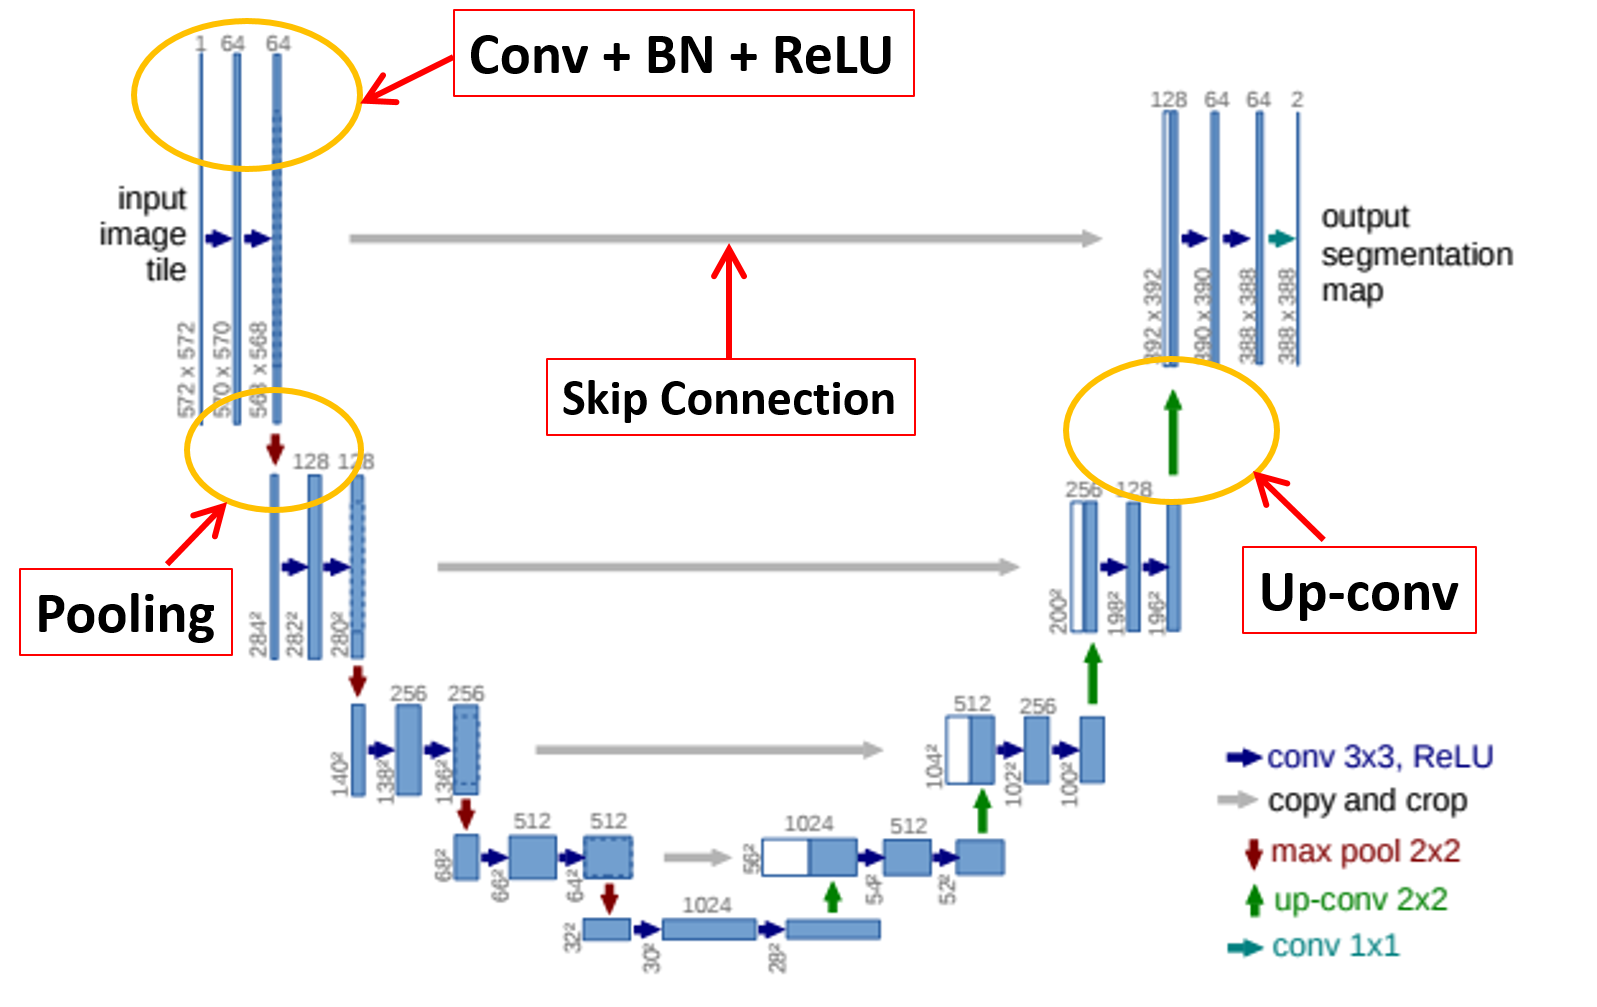
\includegraphics[width=0.8\textwidth]{unet_detailed.png}
		}
	\end{figure}
\end{frame}

\begin{frame}
	\frametitle{Convolution and Convolution Layer \\(\textcolor{pink}{\textbf{Conv}} + BN + ReLU)}
	\textit{Keywords} in Convolution: $\bullet$ \textbf{Kernel Size} \quad $\bullet$ \textbf{Stride} \quad $\bullet$ \textbf{Padding} 
	\begin{figure}[H]
	\centerline{
		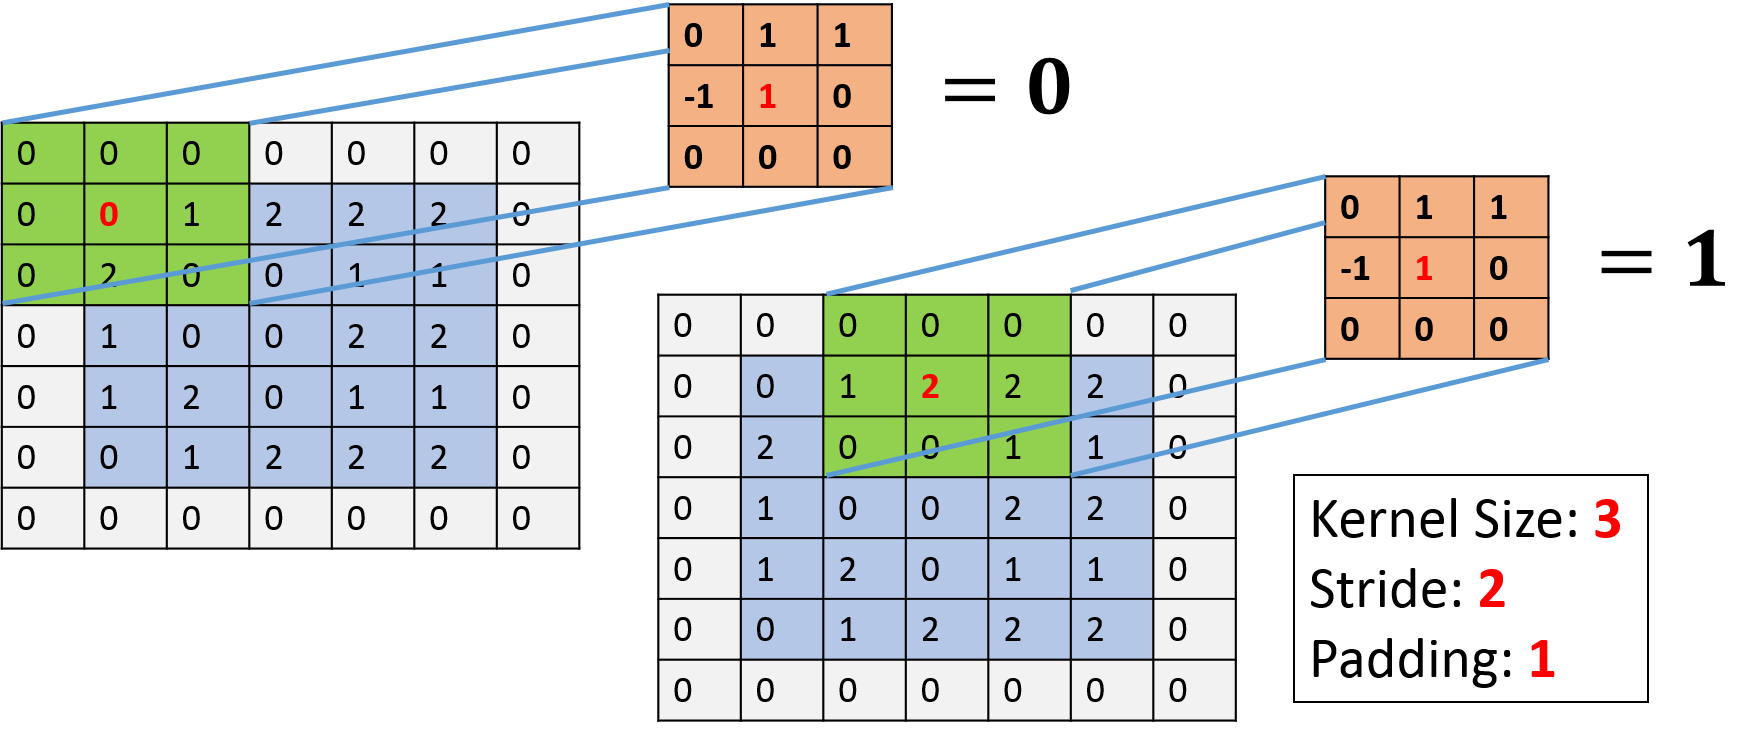
\includegraphics[width=1.0\textwidth]{convolution.png}
	}
	\caption{Illustration of Convolution\footnote{To make it simple, the kernel is already \textbf{rotated}. Only point-wise product and summation is needed}.}
	\end{figure}	
\end{frame}

\begin{frame}
	\frametitle{Convolutions in CNNs: (\textcolor{pink}{\textbf{Conv}} + BN + ReLU)}
	Different types of convolutions. 
	\begin{itemize}
		\item \textbf{Convolution}: (with/without) padding, (1/$>1$) stride.
		\item \textbf{Transposed  Convolution (Deconvolution)}: (with/without) padding, (1/$>1$) stride.
		\item \textbf{Dilated Convolution}.
	\end{itemize}
	\vskip 0.2in
	See the attached HTML file. 
	\vskip 0.2in
	Helpful reading: \textcolor{mycite2}{Vincent Dumoulin, Francesco Visin.} \textit{A guide to convolution arithmetic for deep learning. }
\end{frame}

\begin{frame}
	\frametitle{Convolutional Layer (1st): (\textcolor{pink}{\textbf{Conv}} + BN + ReLU)}
	\begin{figure}[H]
	\centerline{
		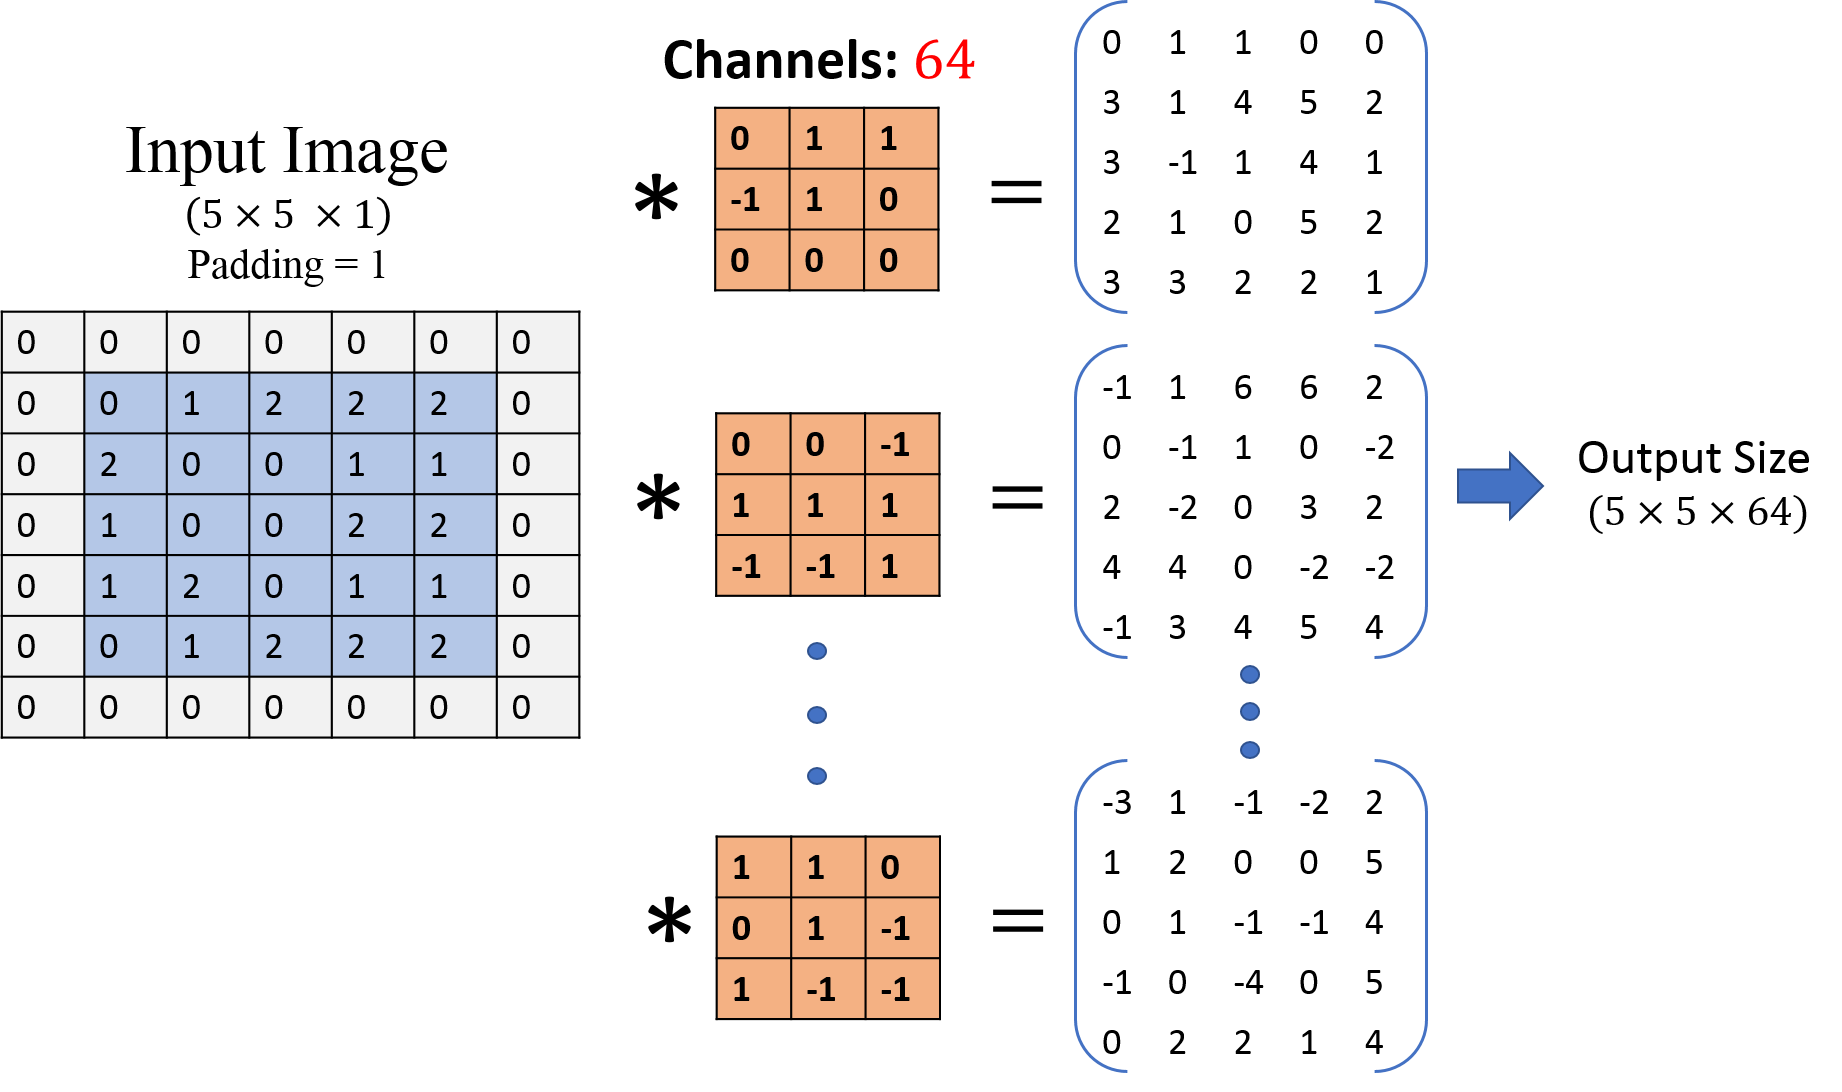
\includegraphics[width=1.0\textwidth]{convolution_1st_layer.png}
	}
	\caption{First Layer of CNN\footnote{Again, all the kernels are already \textbf{rotated}. Only point-wise product and summation is needed.}.}
	\end{figure}		
\vskip -0.2in
\end{frame}

\begin{frame}
\frametitle{Convolutional Layer (2nd): (\textcolor{pink}{\textbf{Conv}} + BN + ReLU)}
	\begin{figure}[H]
		\centerline{
			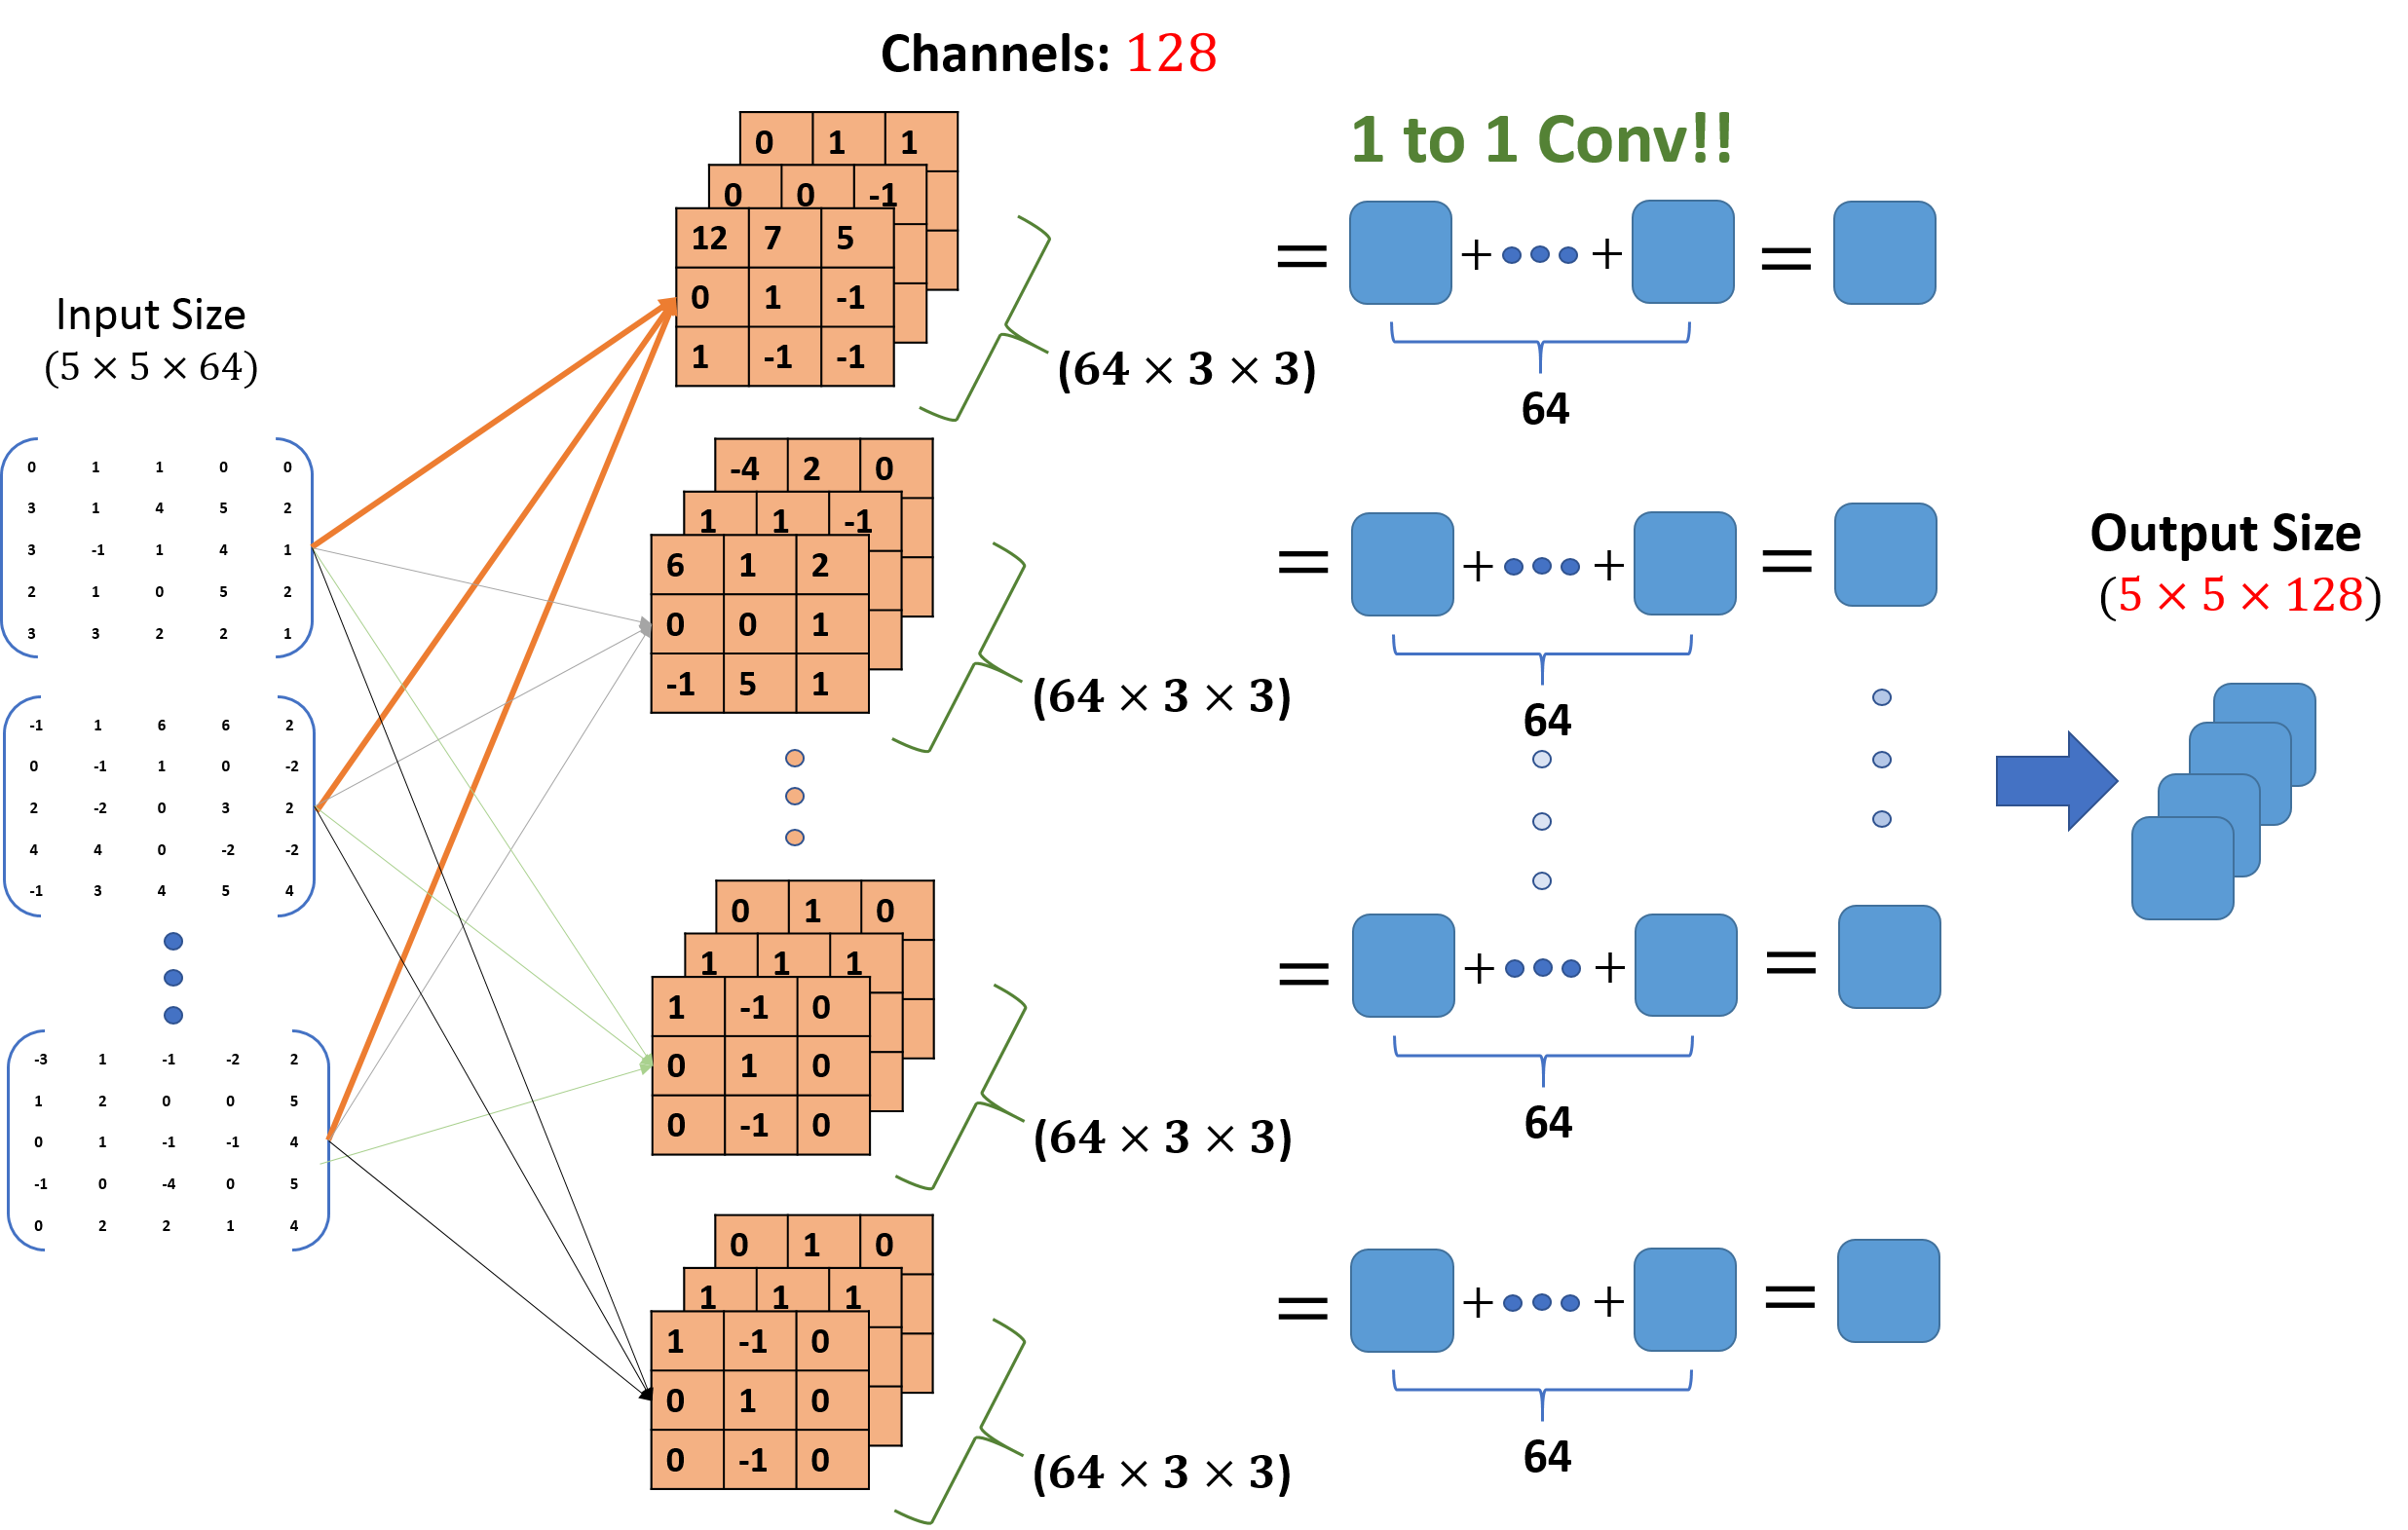
\includegraphics[width=1.0\textwidth]{convolution_2nd_layer2.png}
		}
	\caption{Each channel has 64 different $3\times 3$ filters. Each filter convolves with only \textit{one} channel of the input feature map!}
	\end{figure}
\end{frame}

\begin{frame}
\frametitle{A Short Break: A few questions ...}
Suppose we have $4 \times 512 \time 512 \times 1$ image as network input. That is, (batch size) 4 images where each of them is $512 \times 512 \times 1$ (gray images). Then,
\begin{itemize}
	\item how many parameters (numbers in filters) do we have so far for the first two layers?
	\pause
	\begin{itemize}
		\item $64\times 3 \times 3 + 128\times 64 \times 3 \times 3 = 576 + 73728 = 74,304$
	\end{itemize}
	\pause
	\item since both the batches, feature maps are stored in memory, how much memory do we need? (suppose padding $= 1$, stride $ = 1$)
		\begin{align*}
		&4 \times 512 \times 512 \times 1 + 4 \times 512 \times 512 \times 64 + 4 \times 512 \times 512 \times 128 \\
		&\approx 1M + 67M + 134M = 202M \\
		&= 202 M \times 4\text{ bytes} \approx 770 \text{MB} \quad \text(202M\times4/1024^2)
		\end{align*} 
	\textbf{Some background.} Almost all deep learning models are trained on GPUs. A typical GPU now has $6 \sim 8$ GB memory. Advance GPUs has $12$ GB memory (\eg \text{ } Nvidia GeForce GTX TITAN Z $\sim \$1.5K$ on amazon). 
\end{itemize}

\end{frame}
\begin{frame}
\frametitle{Batch Normalization (Conv + \textcolor{pink}{\textbf{BN}} + ReLU)}
In practice, to increase the training as well as testing speed, we usually feed \textbf{multiple} images to the network. The following figure shows a training batch of 4 images,
	\begin{figure}[H]
		\centerline{
			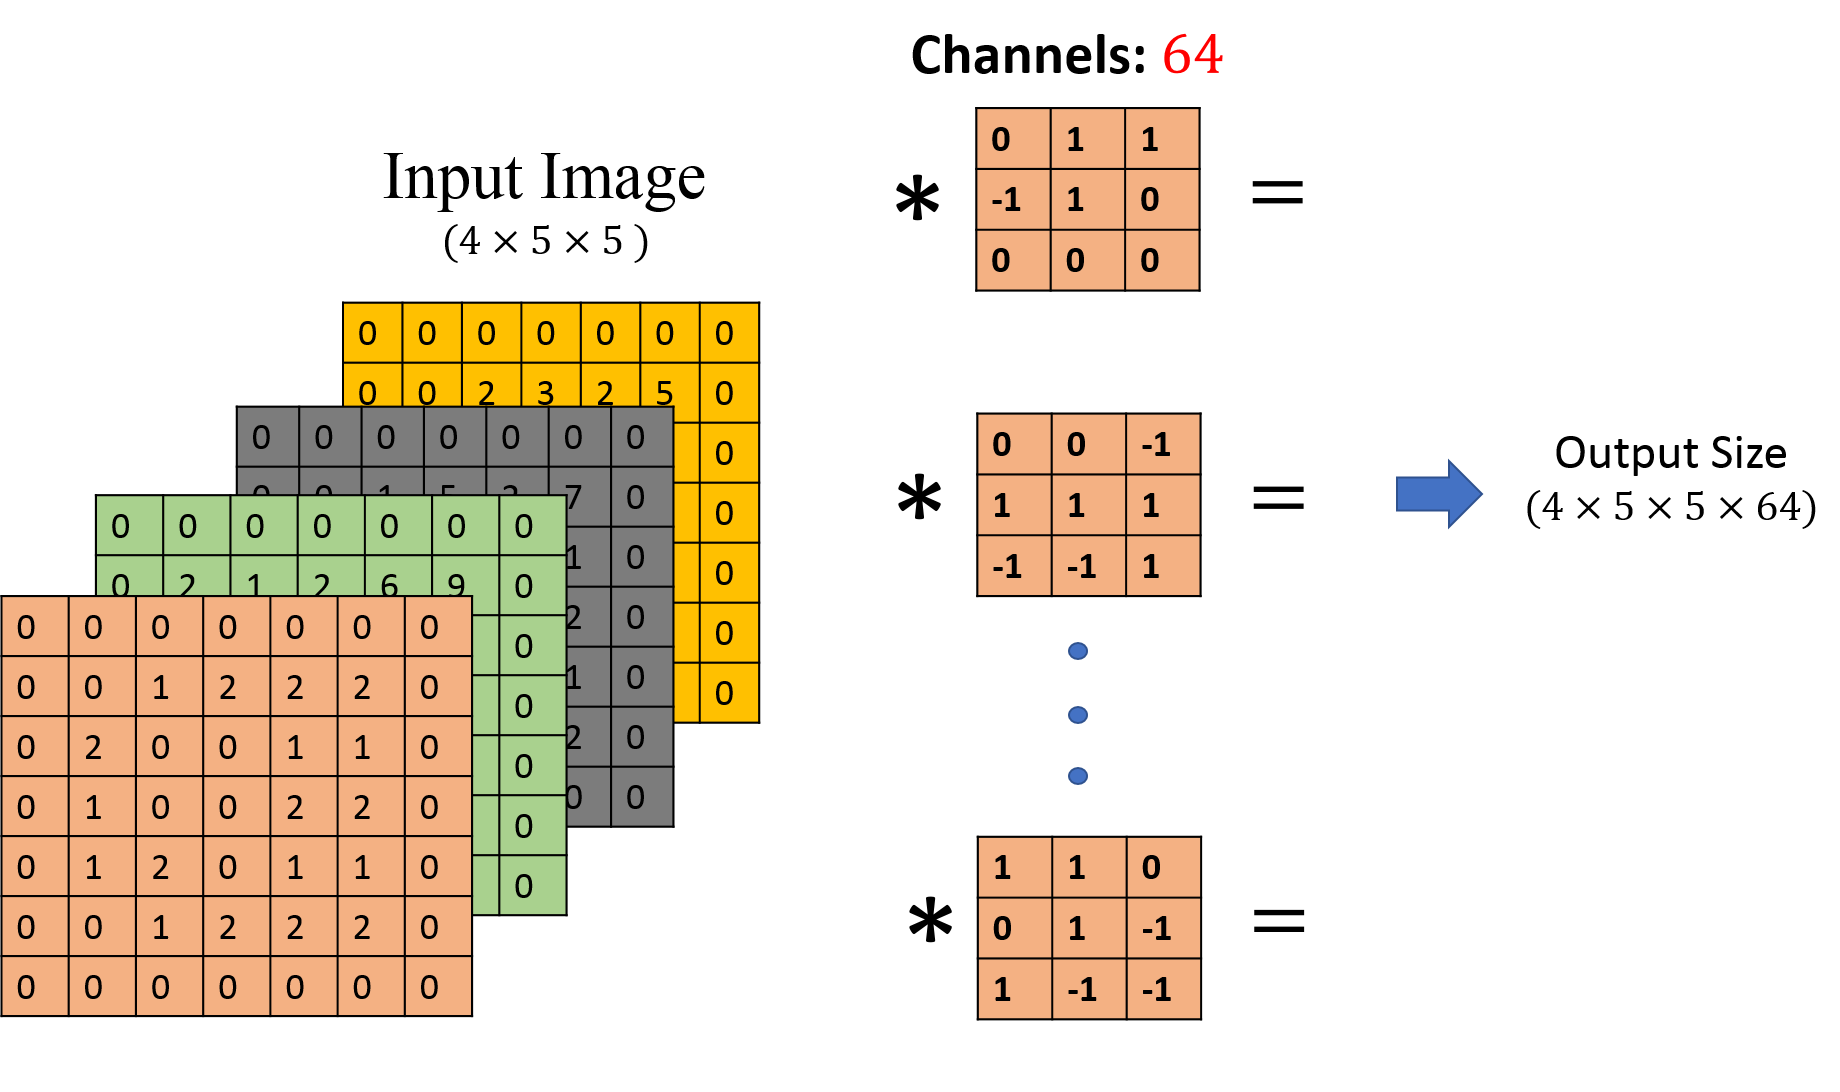
\includegraphics[width=0.9\textwidth]{batch.png}
		}
		\caption{Batch Size is 4. Each Image is independently processed.}
	\end{figure}
\end{frame}


\begin{frame}
	\frametitle{Batch Normalization \blfootnote{\textcolor{mycite2}{Sergey Ioffe, Christian Szegedy}.\textit{ Batch Normalization: Accelerating Deep Network Training by Reducing Internal Covariate Shift}, NIPs 2015.}: (Conv + \textcolor{pink}{\textbf{BN}} + ReLU)}
	For each \textbf{\textit{channel}}, normalize the layers. Mean bad variance are computed across all the values in each channel.
	\begin{figure}[H]
	\centerline{
		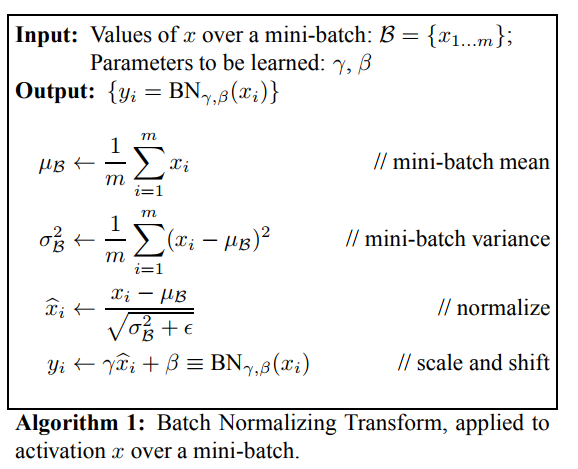
\includegraphics[width=0.6\textwidth]{BN.png}
	}
	\end{figure}	
\vskip -0.3in
	An effective way to resolve \textbf{\textit{vanishing gradient}} problem! 
\end{frame}

\begin{frame}
\frametitle{Nonlinear Activations: (Conv + BN + \textcolor{pink}{\textbf{ReLU}})}
Popular nonlinearities used through all \textbf{but} last layer:
\begin{itemize}
	\item ReLU: $\max (0, x)$.
	\item Leaky ReLU: $\max(0,x) + \gamma^2 \min(0,x)$
	\item Tanh: $\frac{\exp(x) -\exp(-x)}{\exp(x) + \exp(-x)}$
	\item Others \footnote{A good place to find all these is the document of deep learning software frameworks, eg. \url{http://pytorch.org/docs/master/nn.html}}: ELU, SELU, PRELU, Threshold \etc
\end{itemize}
	\begin{figure}
		\centering
		\subfloat[ReLU]{
			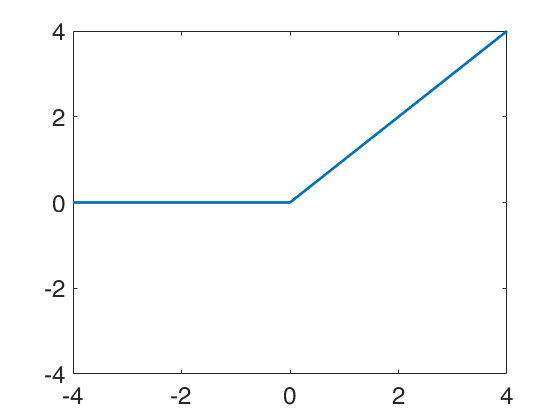
\includegraphics[width=0.33\textwidth]{relu.png}}
		\subfloat[Leaky ReLU]{
			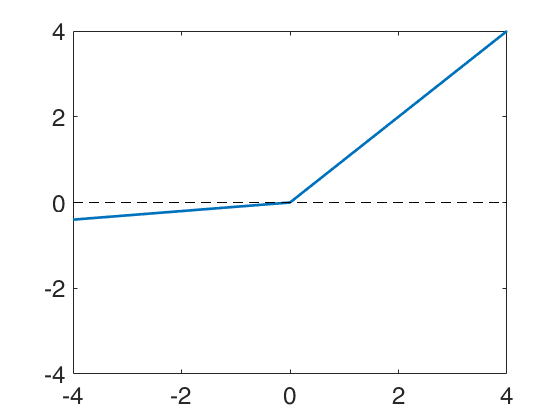
\includegraphics[width=0.33\textwidth]{lrelu.png}}
		\subfloat[Tanh]{
			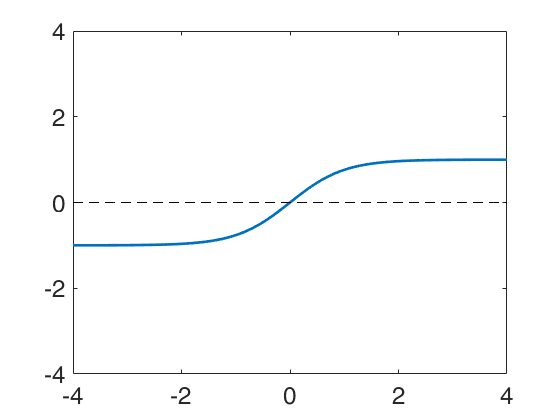
\includegraphics[width=0.33\textwidth]{tanh.png}}
	\end{figure}
\end{frame}

\begin{frame}
\frametitle{Pooling}
	\begin{figure}[H]
	\centerline{
		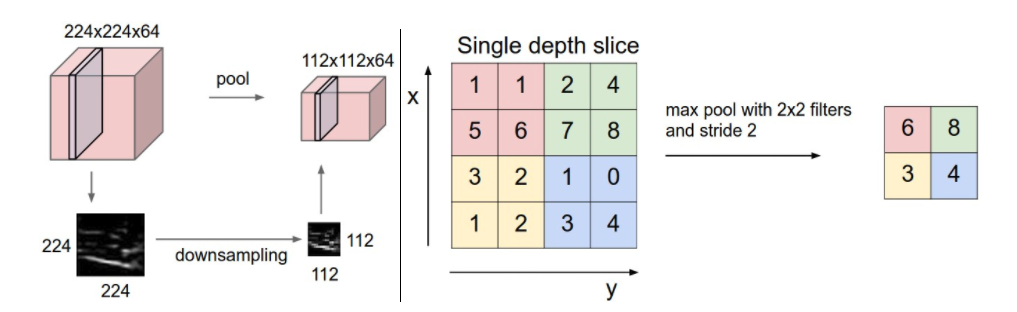
\includegraphics[width=1.0\textwidth]{pooling.png}
	}
	\caption{Illustration of \textit{Max Pooling}. Here batch size 1 is omitted. \footnote{Image courtesy of  CS231n: Convolutional Neural Networks for Visual Recognition.  Stanford.}}
	\end{figure}
	There is also average pooling which takes average rather than maximum.
\end{frame}

\begin{frame}
	\frametitle{Skip Connection}
	\begin{figure}[H]
	\centerline{
		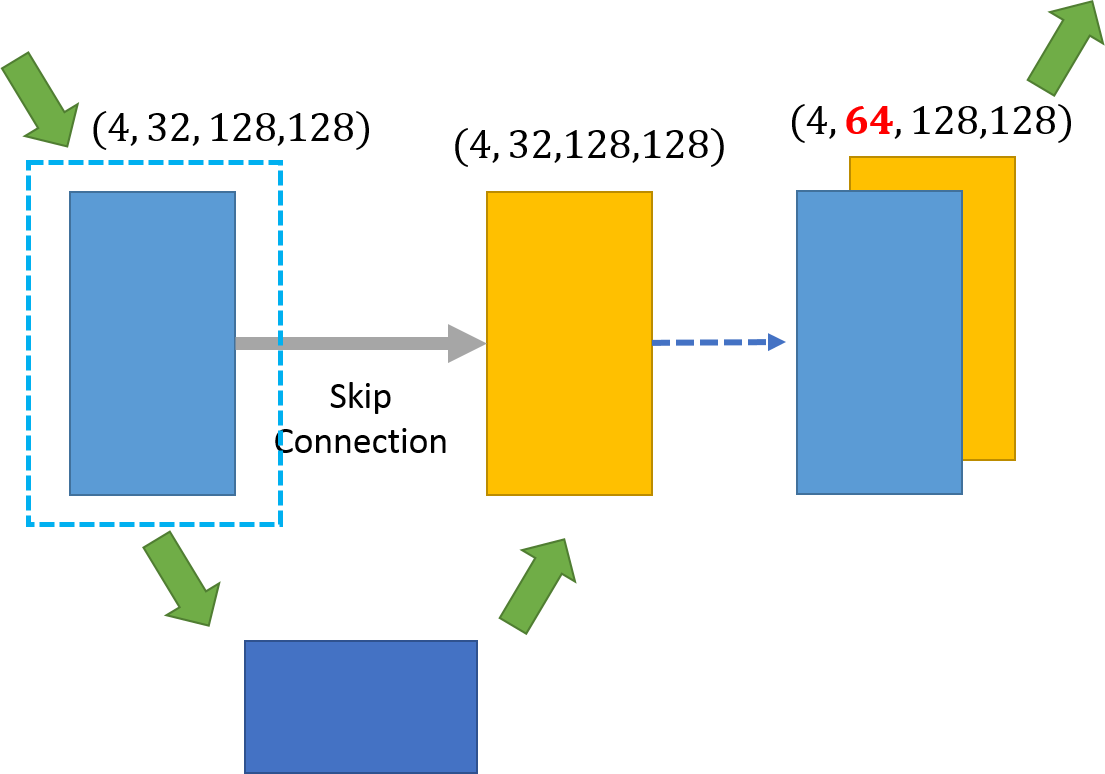
\includegraphics[width=0.6\textwidth]{skip.png}
	}
	\caption{Skip connection is simply concatenating two feature maps (along channel dimension). Central crop is performed is there is a miss-match of the dimension.}
	\end{figure}	
\vskip -0.2in 
	\textbf{Comment.} Adding skip connections can usually increase the performance (at least) in segmentation.
\end{frame}

\begin{frame}
\frametitle{Dense Layer}
	\begin{figure}[H]
	\centerline{
		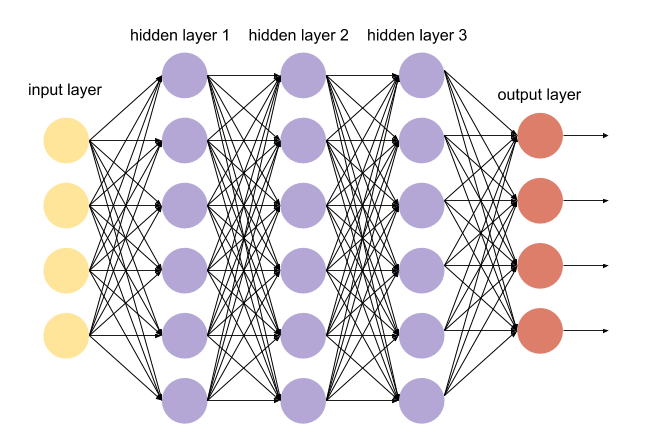
\includegraphics[width=1\textwidth]{denselayer.png}
	}
	\caption{Dense Layers}
\end{figure}
\end{frame}
\begin{frame}
\frametitle{Now We Know ($+-\times \div$) ...}
	\begin{figure}[H]
	\centerline{
		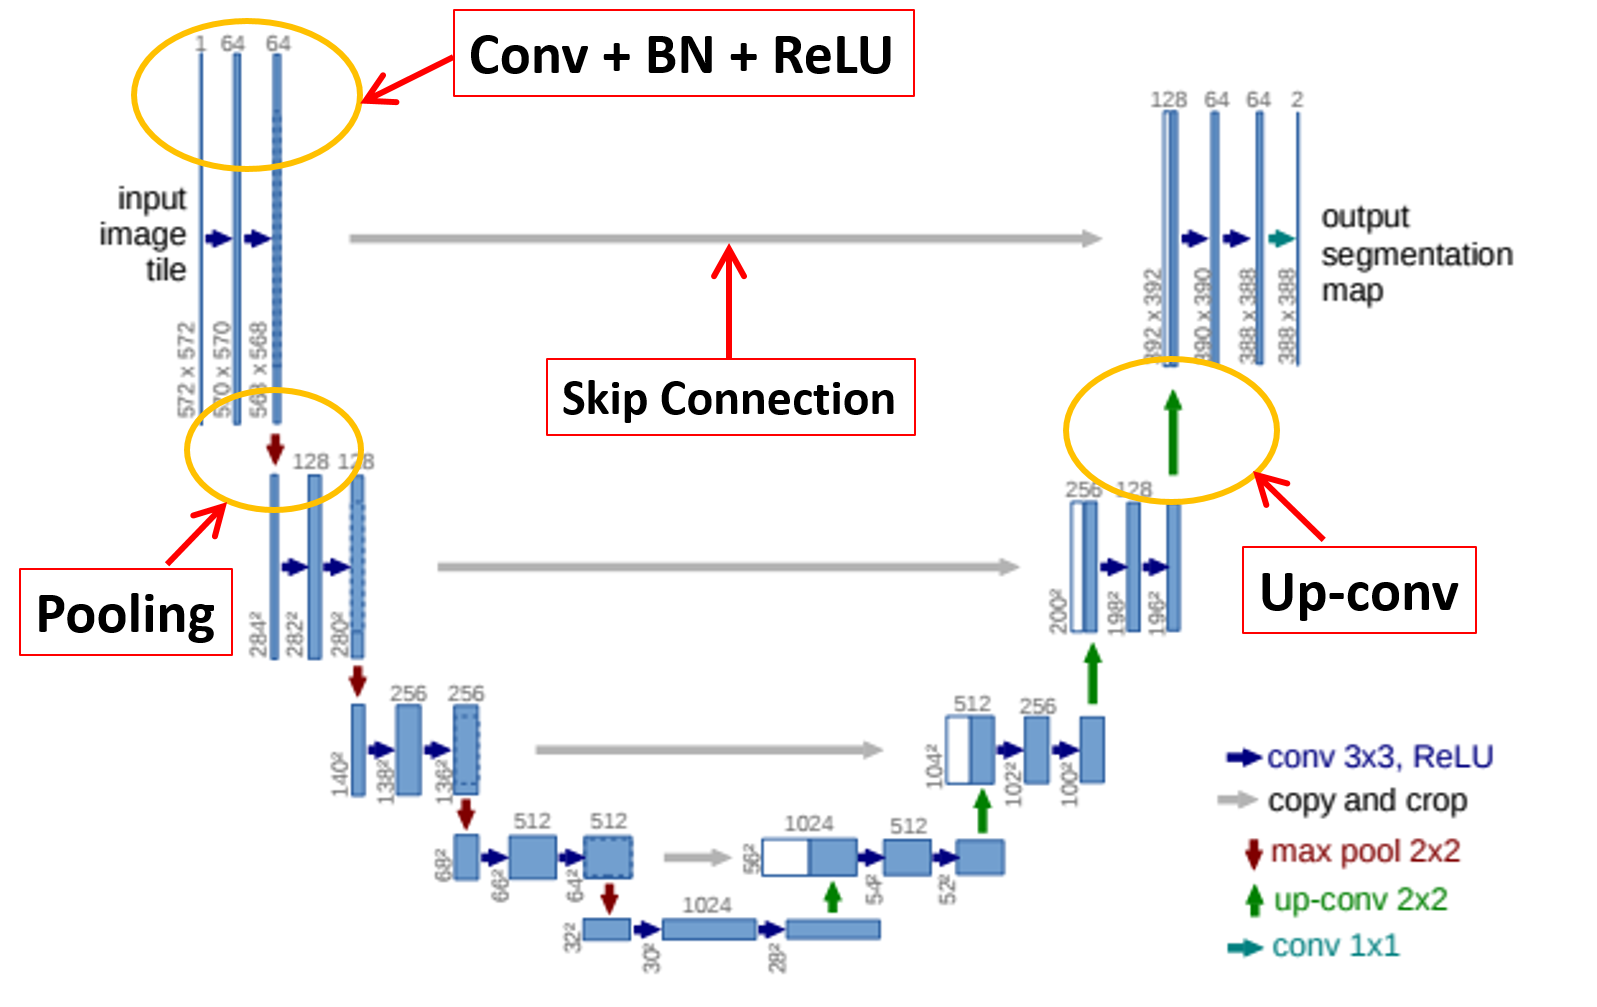
\includegraphics[width=0.8\textwidth]{unet_detailed.png}
	}
	\caption{Networks are just special ways to stack all these operations.}
\end{figure}
\end{frame}


\subsection{Optimization Problems in CNNs}
\begin{frame}
\frametitle{Function Representation}
	\begin{figure}[H]
	\centerline{
		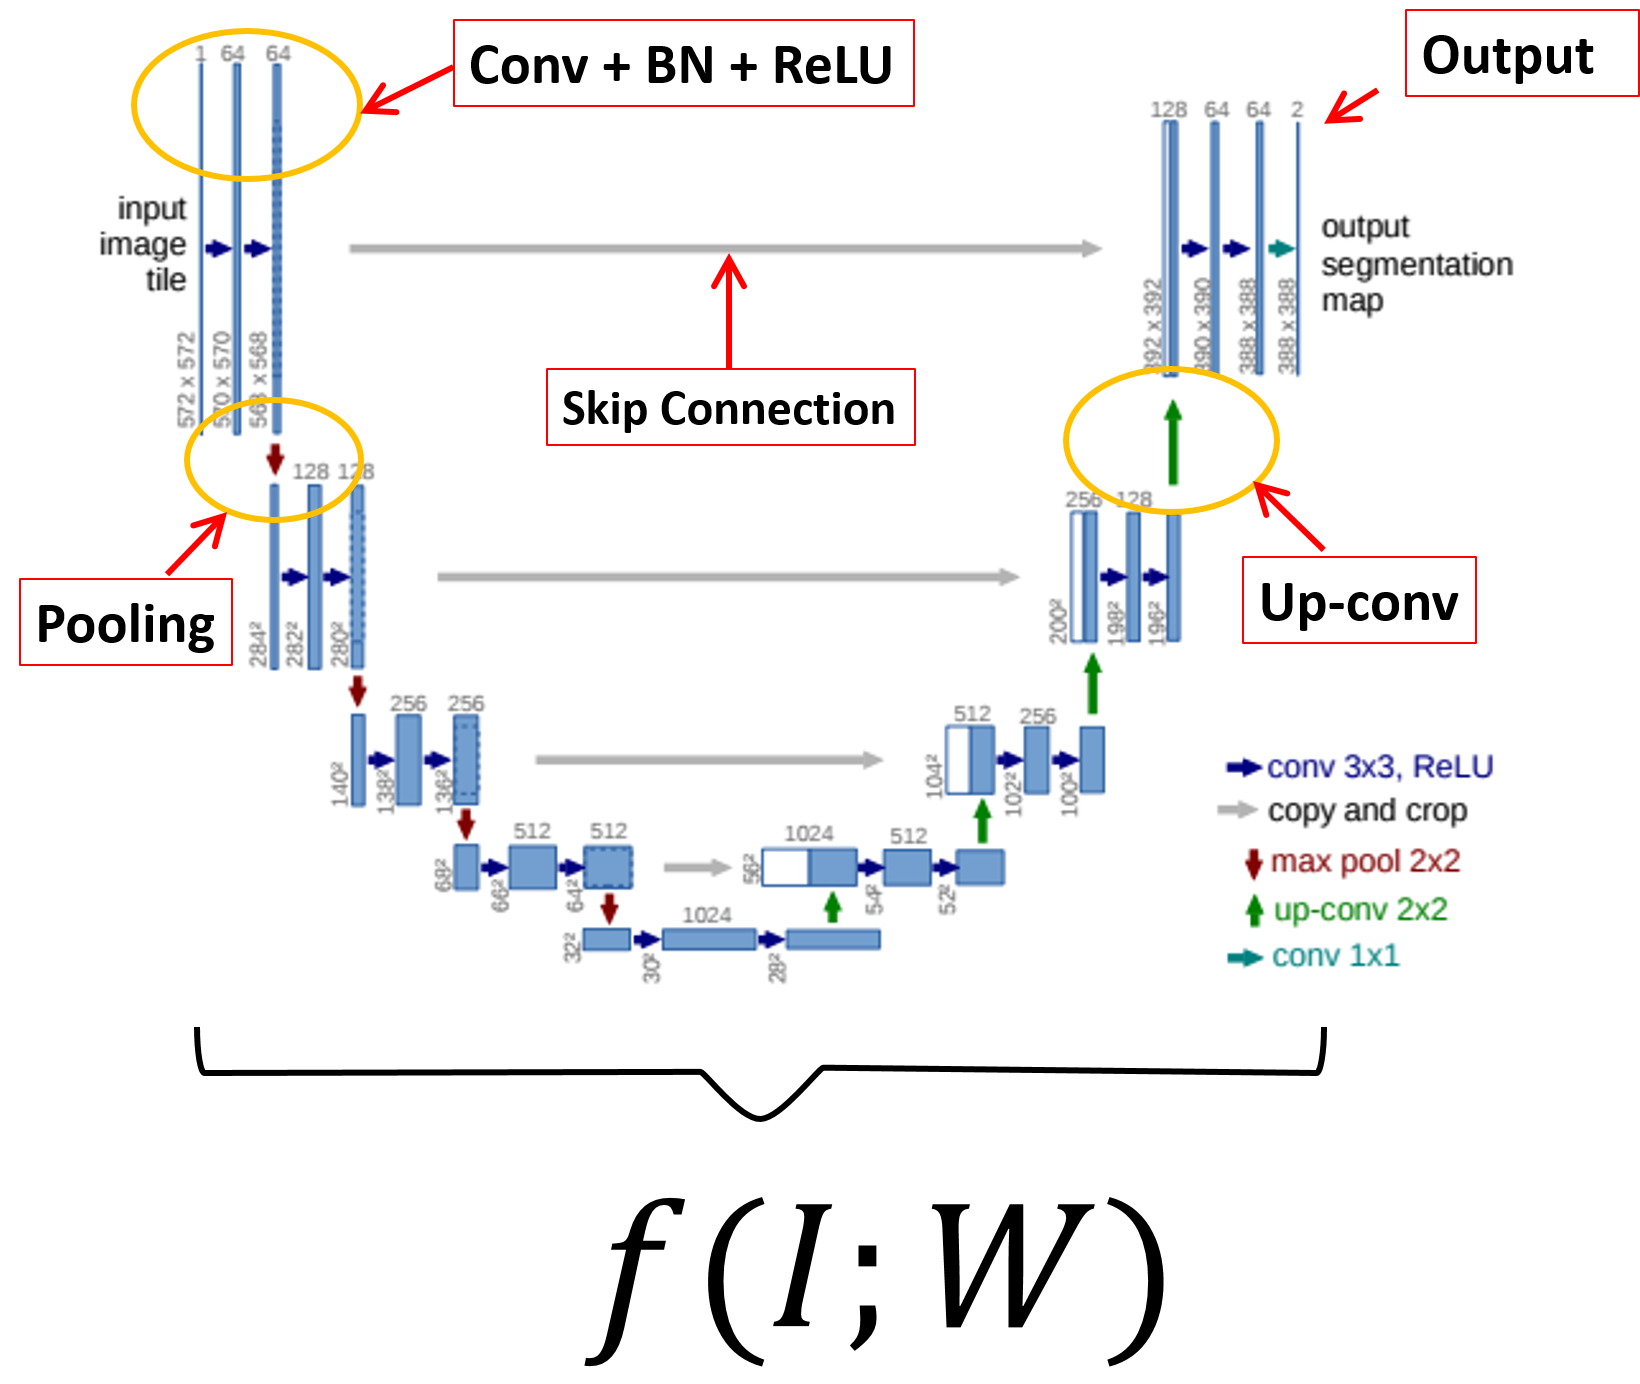
\includegraphics[width=0.6\textwidth]{optimization_fx.png}
	}
	\caption{The entire network is just another representation of $f(I; W)$, where $I$ is input image(s), $W$ are the parameters in the network.}
	\end{figure}
\end{frame}


\begin{frame}
\frametitle{The Logics of Deep Learning (Supervised Training)}
	\begin{figure}[H]
	\centerline{
		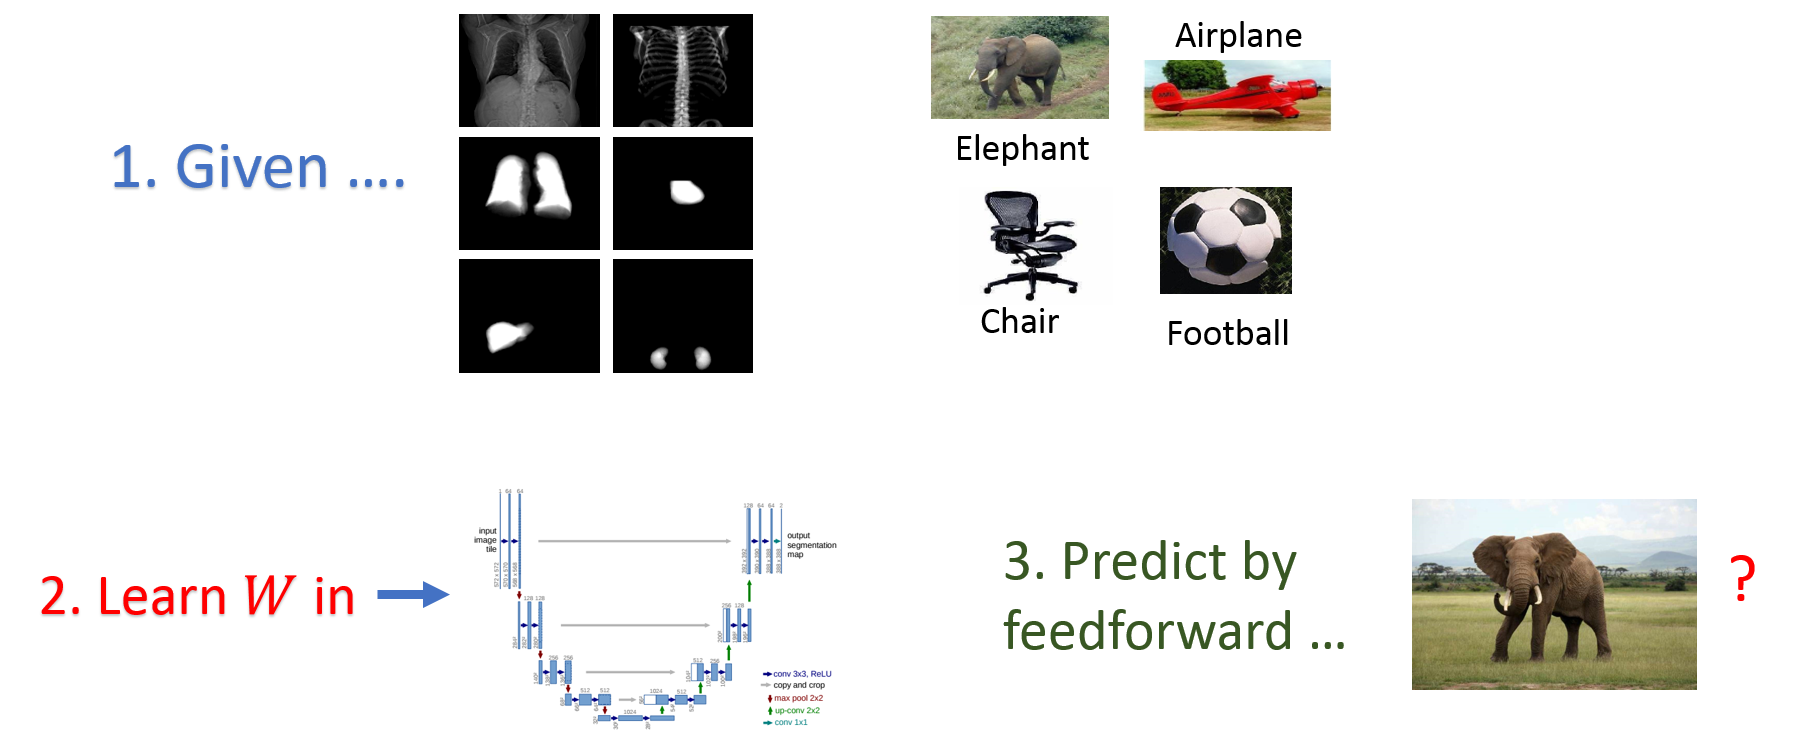
\includegraphics[width=1\textwidth]{logics.png}
	}
\caption{Working Logics of Supervised Deep Learning. (Training vs. Testing)}
	\end{figure}

A standard workflow includes training $\rightarrow$ validation $\rightarrow$ testing.
\end{frame}

%===============================================================================

\begin{frame}
\frametitle{Optimization Problem}
In training state, we are given ground truth images and its labels for recognition/classification, or masks for segmentation, high-resolution image for super-resolution, clear image for de-noising \etc. 
\vskip 0.2in
Let $I$ be the truth images and $g$ be their labels, the optimization problem is 
\[
\min_W \quad Loss\{ f(I; W) - g\}
\] 
Popular losses,
\begin{itemize}
	\item \textbf{$l_2$ distance}: image denoising, super-resolution, recognition.
	\item \textbf{Entropy}: binary/categorical cross-entropy, KL-divergence for segmentation.
	\item Many other \textbf{customized losses}, \eg \text{ } $l_1$ for GAN, smoothed dice loss for segmentation.
\end{itemize}
\end{frame}

\begin{frame}
\frametitle{Loss Function Example: Cross Entropy}
	\begin{figure}[H]
	\centerline{
		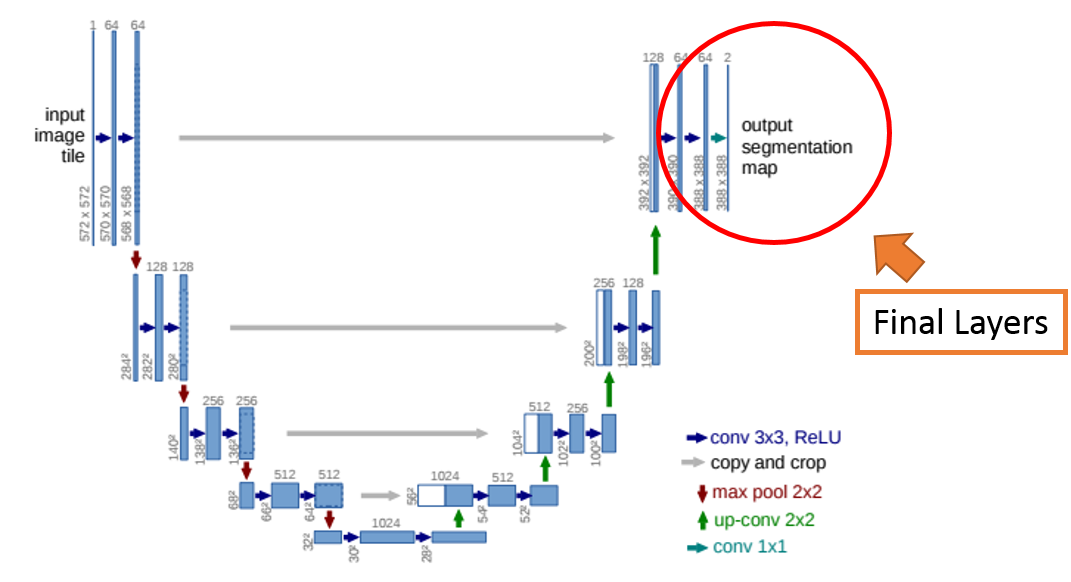
\includegraphics[width=1\textwidth]{loss_last_layer.png}
	}
	\caption{Let's look at what happens at the last layer (for single-object segmentation).}
	\end{figure}
\end{frame}

\begin{frame}
\frametitle{Loss Function Example: Cross Entropy}
Suppose we are doing a single object segmentation, \eg\ lung. The last convolutional channel will have 2 channels corresponding foreground and background. 
	\begin{figure}[H]
	\centerline{
		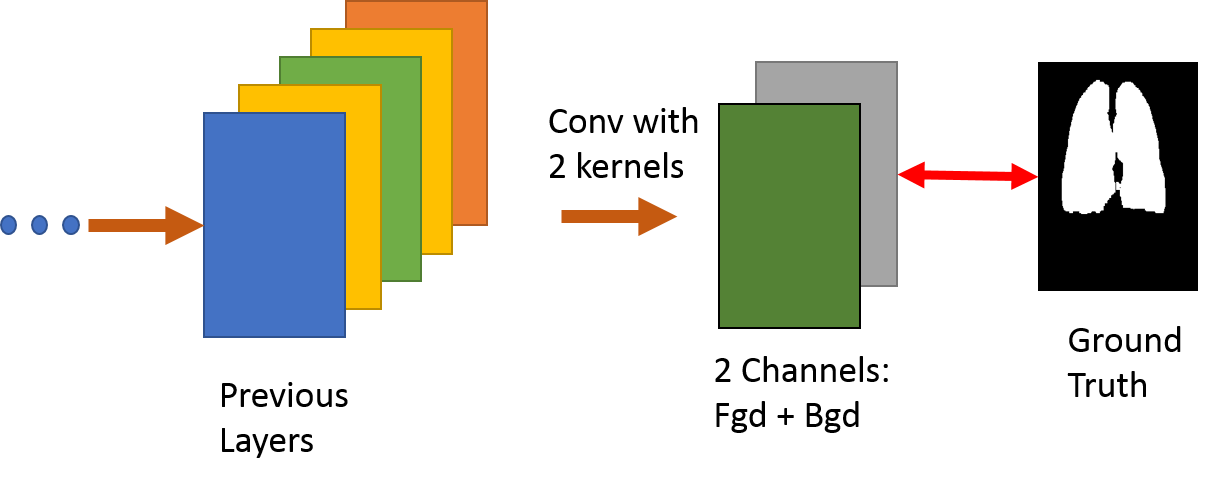
\includegraphics[width=0.8\textwidth]{last_layer.png}
	}
	\caption{\textbf{Loss = Softmax + Cross-entropy}}
	\end{figure} 
\end{frame}

\begin{frame}
\frametitle{Loss Function Example: Cross Entropy}
Let $A = (F, B) \in \R^{256\times 256 \times 2}$ be the output map with $F \in \R^{256\times 256}$ and $B \in \R^{256 \times 256}$ are the foreground and background channels. 
\begin{itemize}
	\item Softmax: 
	\[
	S := Softmax(A)_{ij} = \frac{\exp(F_{ij})}{\exp(F_{ij}) + \exp(B_{ij})}
	\]
	\item Final Cross Entropy Loss:
	\begin{align*}
	\mathcal{L} = -\bigg(\frac{1}{256^2}\sum_{i=1}^{256} \sum_{j=1}^{256}y_{ij} \log(S_{ij}) + (1-y_{ij}) \log(1-S_{ij})\bigg)
	\end{align*}
	where $y_{ij}$ is 1 if the pixel belongs to lung and 0 otherwise.
\end{itemize}
In \textbf{testing} phase, the prediction mask will be a simple comparison between foreground and background.
\end{frame}

\begin{frame}[fragile]
\frametitle{Code Samples}
Code samples of Conv-BN-ReLU.
\begin{lstlisting}[language=Python,keywordstyle=\color{red}]
net['conv0_1'] = batch_norm(
Conv2DDNNLayer(net['input'], 
num_filters=64, filter_size=3, pad='same', 
W=HeNormal(gain='relu'), nonlinearity=rectify))

net['conv0_2'] = batch_norm(
Conv2DDNNLayer(net['conv0_1'], num_filters=64, 
filter_size=3, pad='same',
W=HeNormal(gain='relu'), nonlinearity=rectify))
\end{lstlisting}

\end{frame}


\section{Optimization in Deep Learning}
\begin{frame}
	\frametitle{Optimization Routine of Deep Networks}
	The optimization of $W$ is based on gradient descent algorithm.
	\begin{enumerate}
		\item Initialize the weights  of the entire network as $W_0$, a learning rate $\alpha$.
		\item For $k = 1,2, ...$
		\begin{enumerate}
			\item Update $W_k$: $W_k = W_{k-1} - \alpha \nabla_W L(I;W_{k-1})$.
			\item if $mod(k, 10K) == 0$: $\alpha \leftarrow 0.8*\alpha$.
		\end{enumerate}
		\item Select the best iterations by cross-validation.
	\end{enumerate}
So, how can we calculate $\nabla_W L(I;W_{k-1})$?
\end{frame}


\begin{frame}
\frametitle{Backpropagation In Convolutional Neural Networks}
Function $f(I;W)$ can be written as a series composition of operations, that is
\[
f(\cdot;W) = C_n  \circ \cdots  C_2 \circ  P_1 \circ R_1 \circ B_1 \circ C_1 \circ I_d
\]
where $I_d$ is identity, $C-B-R$ is conv-bn-relu, $P$ is pooling. (Recall transposed convolution is also convolution, it therefore belongs to this general setting).
For simplicity, consider the $l_2$ loss,
\[
L = \frac{1}{2} \|f(I;W) - g\|_2^2
\] 
The gradient descent method requires the access to $\frac{\partial L}{\partial W}$, which is,
\begin{align*}
\frac{\partial L}{\partial W} &= \frac{\partial f}{\partial W} (f-g) \\
&= \frac{\partial }{\partial W}(C_n  \circ \cdots \circ B_1 \circ C_1 \circ I_d) (f-g)
\end{align*}
\end{frame}


\begin{frame}
\frametitle{Chain Rule}
Recall the chain rule:
\[
(f\circ g) ' = (f'\circ g ) \cdot g' \quad \text{ for }    f(x), g(x)
\]
Or (with variable replacing trick).
\[ \frac{dz}{dx} = \frac{dz}{dy} \cdot  \frac{dy}{dx}  \quad \text{ for } z=f(y), y=g(x)
\]
And a straightforward consequence,
\[ 
\frac{df}{dW} = \frac{df}{dC_n} \cdot  \frac{dC_n}{dP_{n-1}} \cdot  \frac{dP_{n-1}}{dR_{n-1}} \cdots \frac{dC_1}{dI} \quad \text{ for }  f = f(I;W)
\]
We now study each of the factors, and a final output will be the products.
\end{frame}

%\begin{frame}
%\frametitle{Backpropagation on Convolutions: $\frac{\partial f}{\partial C}$}
%Derivatives of convolutions (easy to be verified by Fourier transforms),
%\[
%(f \ast g) ' =  f' \ast g = f \ast g'
%\]
%\end{frame}

\begin{frame}
\frametitle{Backpropagation on Convolutions: $\frac{\partial f}{\partial C}$}
	\begin{figure}[H]
	\centerline{
		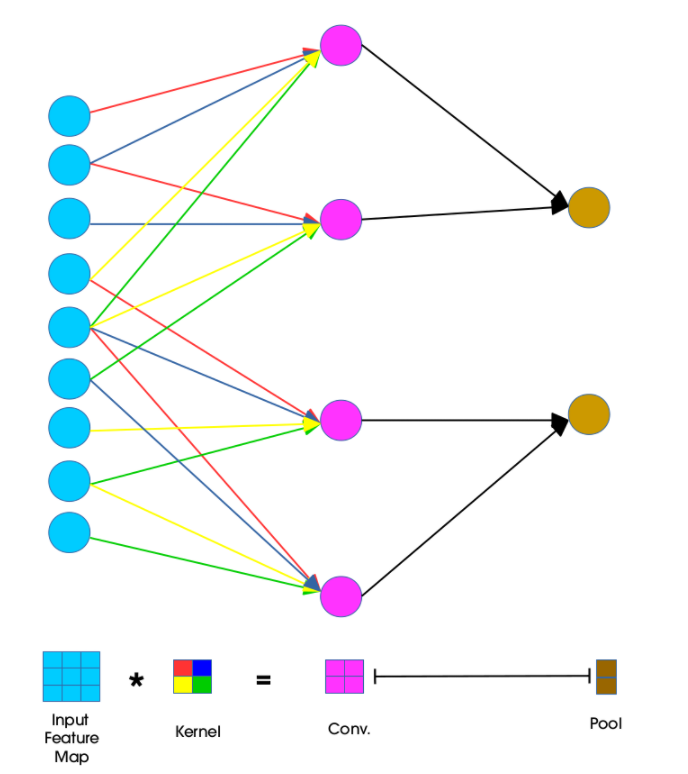
\includegraphics[width=0.6\textwidth]{convolution_forward.png}
	}
	\caption{Convolution layer can be written as `sparse' dense layers.}
	\end{figure}
\end{frame}

\begin{frame}
\frametitle{Backpropagation on Convolutions: $\frac{\partial f}{\partial C}$ \footnote{\url{https://www.slideshare.net/kuwajima/cnnbp}}}
\begin{figure}[H]
	\centerline{
		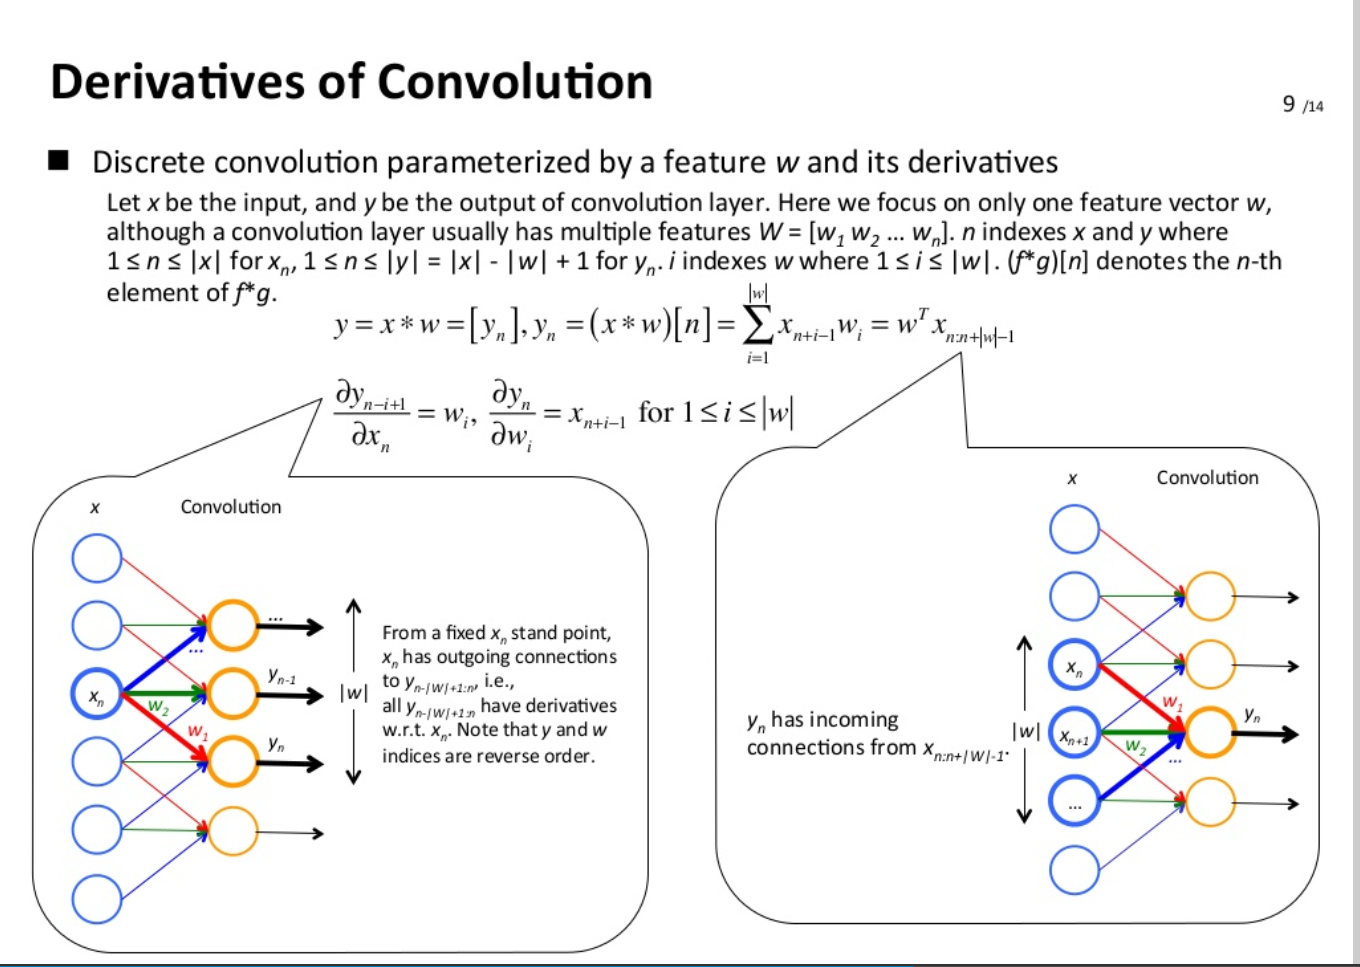
\includegraphics[width=1\textwidth]{back_conv1.png}
	}
\end{figure}
\end{frame}

\begin{frame}
\frametitle{Backpropagation on Convolutions: $\frac{\partial f}{\partial C}$ \footnote{\url{https://www.slideshare.net/kuwajima/cnnbp}}}
\begin{figure}[H]
	\centerline{
		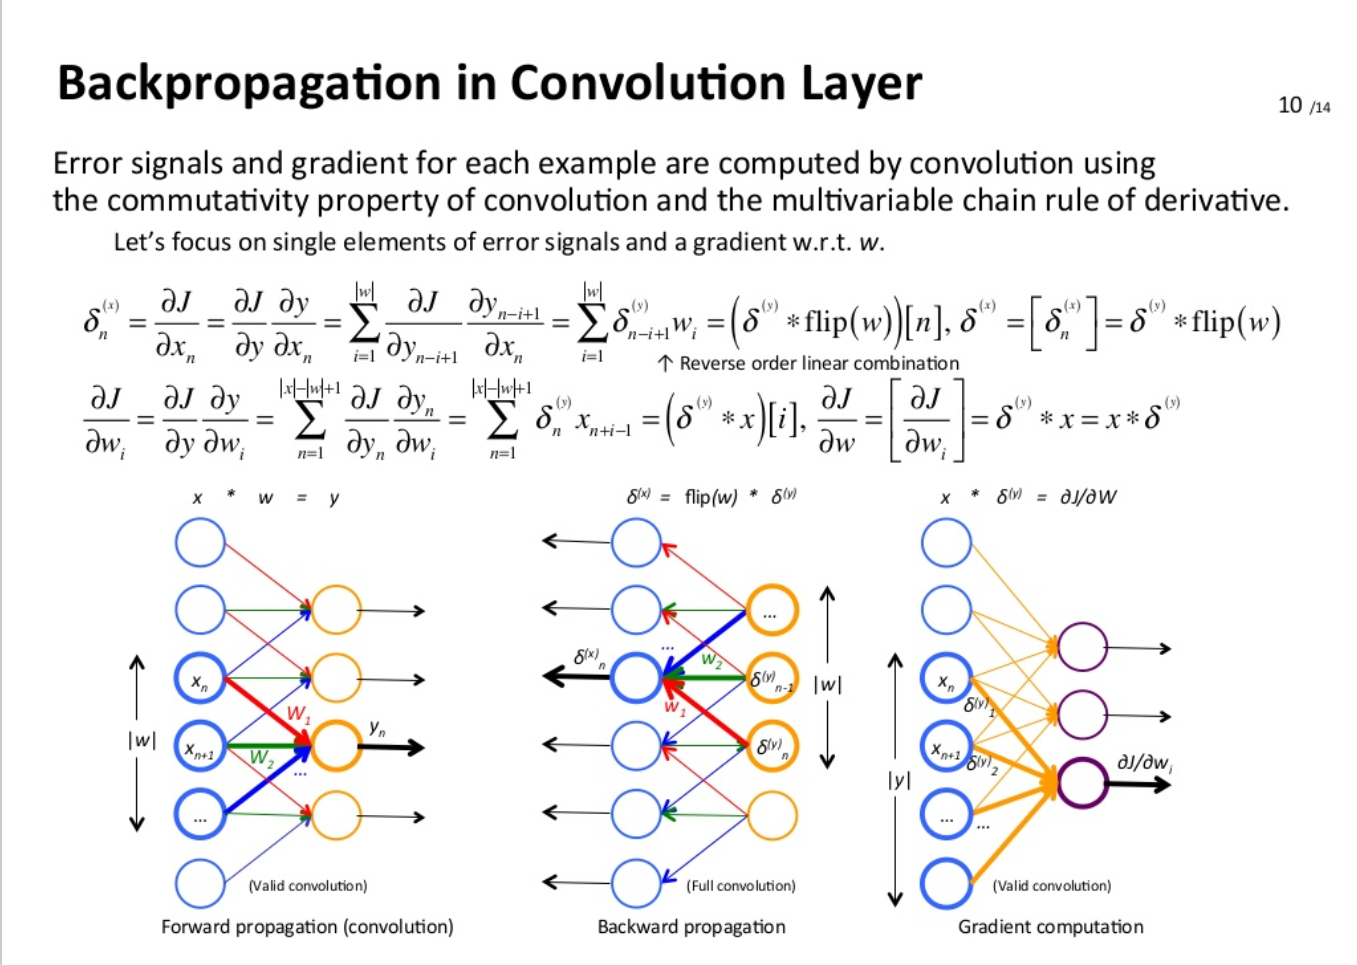
\includegraphics[width=1\textwidth]{back_conv2.png}
	}
\end{figure}
\end{frame}

\begin{frame}
\frametitle{Backpropagation on ReLU and Max-Pooling}
\begin{itemize}
	\item Since $R = \max(0,B)$, the derivative is defined piece-wisely as an indicator function,
	\[
	\frac{\partial R}{\partial B} = \begin{cases} 0 &\mbox{if } B\leq 0 \\ 
	\frac{\partial B}{\partial B} = 1 & \mbox{if } B>0 \end{cases}  
	\]
	\item Recall max-pooling is taking maximum of small neighborhood around each pixel, the derivate of it w.r.t. the previous layer will also be $\delta$ functions!
\end{itemize}
\end{frame}


\begin{frame}
\frametitle{Backpropagation on BN \footnote{\url{https://kevinzakka.github.io/2016/09/14/batch_normalization/}}}
	\begin{figure}[H]
	\centerline{
		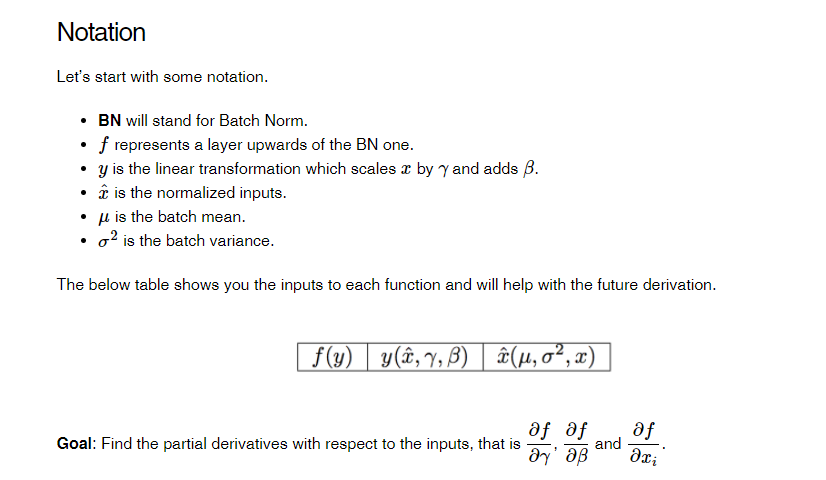
\includegraphics[width=1\textwidth]{back_bn.png}
	}
\end{figure}
\end{frame}



\begin{frame}
\frametitle{Backpropagation on BN \footnote{\url{https://kevinzakka.github.io/2016/09/14/batch_normalization/}}}
\begin{figure}[H]
	\centerline{
		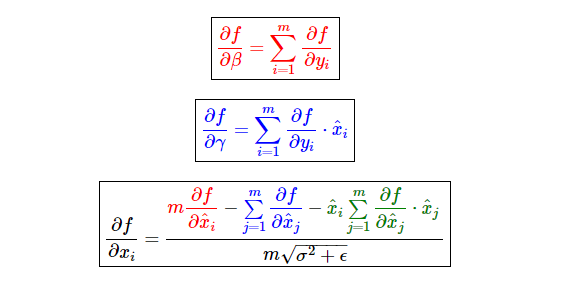
\includegraphics[width=1\textwidth]{back_bn_2.png}
	}
\caption{Details can be found from the link.}
\end{figure}
\end{frame}

\begin{frame}
\frametitle{First Order Methods in Deep Learning Optimization}
Since we can obtain the gradient of $f(I;W)$ from the back-prop, we can minimize the loss using first order methods:
\begin{itemize}
	\item SGD,
	\item Momentum,
	\item Nesterov accelerated gradient,
	\item Adam,
	\item RMSprop,
	\item Adagrad, ...
\end{itemize}
See \url{http://ruder.io/optimizing-gradient-descent/index.html}
\end{frame}

\section{Coding}
\begin{frame}
\frametitle{System/Software Requirements}
\begin{itemize}
	\item Python (preferred 3.0 and later).
	\item Theano + Lasagne:
	\begin{enumerate}
		\item \url{http://deeplearning.net/software/theano/install.html}
		\item \url{https://github.com/Lasagne/Lasagne}
	\end{enumerate}
	\textbf{Or} Pytorch:
	\begin{enumerate}
		\item OSX + Linux: \url{http://pytorch.org/}
		\item Windows: \url{https://github.com/peterjc123/pytorch-scripts}
	\end{enumerate} 
	\item A GPU.
\end{itemize}
\end{frame}


\begin{frame}
\frametitle{Popular Code Schemes}
	\begin{figure}[H]
	\centerline{
		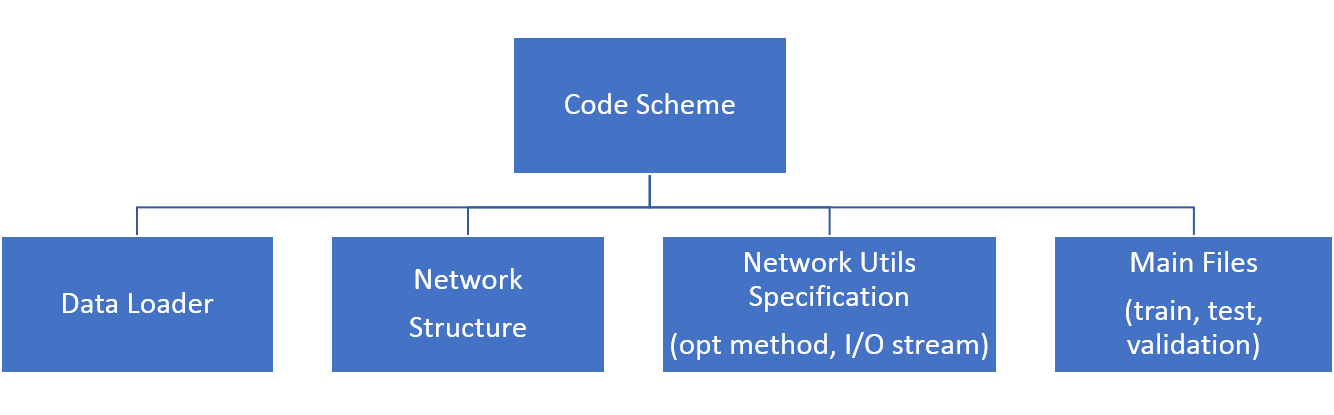
\includegraphics[width=1.0\textwidth]{code_scheme.png}
	}
\end{figure}
Here,
\begin{itemize}
	\item \textbf{Data Loader:} a function file, loads data to (pytorch array);
	\item \textbf{Network Structure:} a function file, specifies network structure (UNet, Densenet \etc);
	\item \textbf{Network Utils Specification:} a function file, specifies optimization methods (adam, sgd, \etc) and input/output stream of the network;
	\item \textbf{Main Files:}  the 3 running files: train, test, validation.  
\end{itemize} 
\end{frame}


\begin{frame}
\frametitle{Data Loader (Pytorch)}
\begin{itemize}
	\item Load data $\rightarrow$ \textbf{augmentation} $\rightarrow$ return augmented images + labels
	\vskip 0.2in
	\item It \textbf{requires} 3 functions:
	\begin{enumerate}
		\item \textbf{init}: initialization
		\item \textbf{getitem}: load data and augmentation
		\item \textbf{len}: size of the data
	\end{enumerate}
\end{itemize}
	\begin{figure}[H]
	\centerline{
		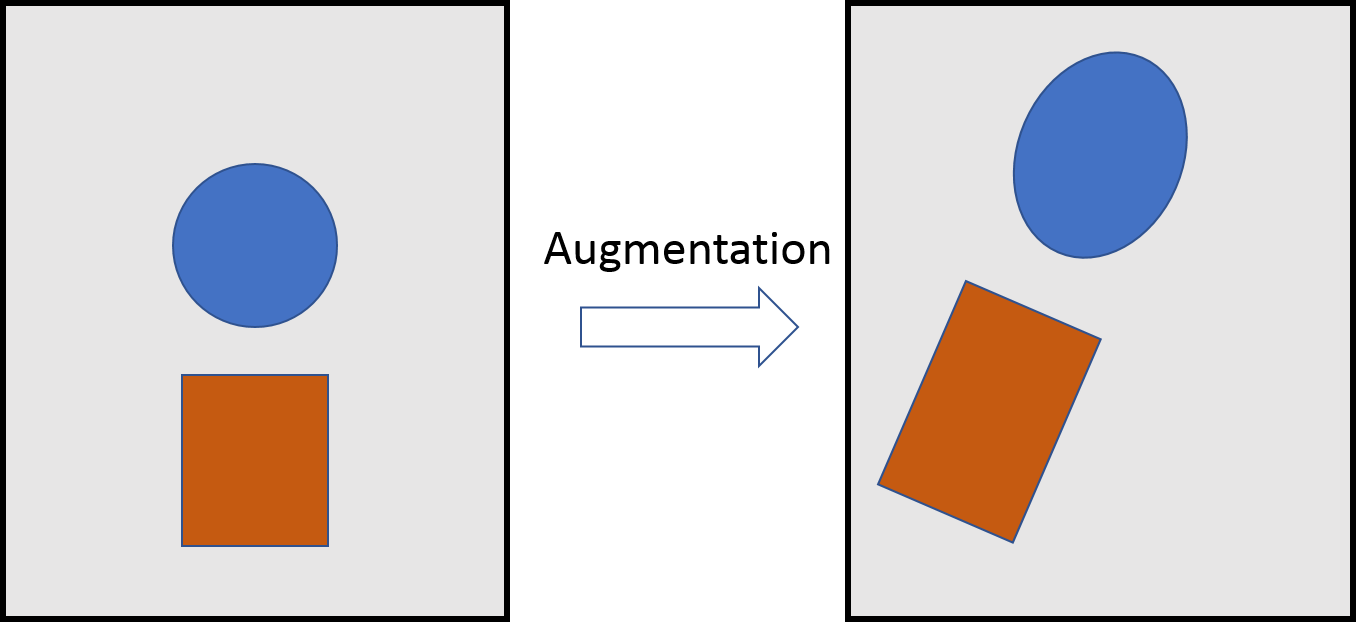
\includegraphics[width=0.5\textwidth]{augmentation.png}
	}\caption{Illustration of Data Augmentation: translation+rotation+scaling}
\end{figure}
\end{frame}

\begin{frame}
\frametitle{Network Structure (Lasagne)}
This file contains the structure of the network: 
\begin{itemize}
	\item different layers: conv/deconv, pooling layer
	\item padding, stride, weight initialization
	\item batch normalization, nonlinear activation.
\end{itemize}
\vskip 0.2in
For Pytorch, a \textbf{forward} function has to be specified.
\end{frame}

\begin{frame}
\frametitle{Networkio (Pytorch)}
This file contains the necessary utility functions:
\begin{itemize}
	\item specifies optimization method (learning rate, parameters),
	\item specifies the loss function and how it is computed,
	\item save the learned parameters to files,
	\item load the learned parameter from files.
\end{itemize}
\end{frame}

\begin{frame}
\frametitle{Main Files (Pytorch)}
Ideally, a program should include 3 main files: 
\begin{itemize}
	\item \textbf{train}: load training data, start training, save weights of each \textbf{epoch}.
	\item \textbf{validation}: load validation data, load the trained weights of each epoch, find the best one.
	\item \textbf{test}: load test data, load the best weights, report the testing accuracy.
\end{itemize}
\end{frame}

\section{Networks Variants: Many More to Explore}
\begin{frame}
\frametitle{Networks}
\begin{figure}[H]
	\centerline{
		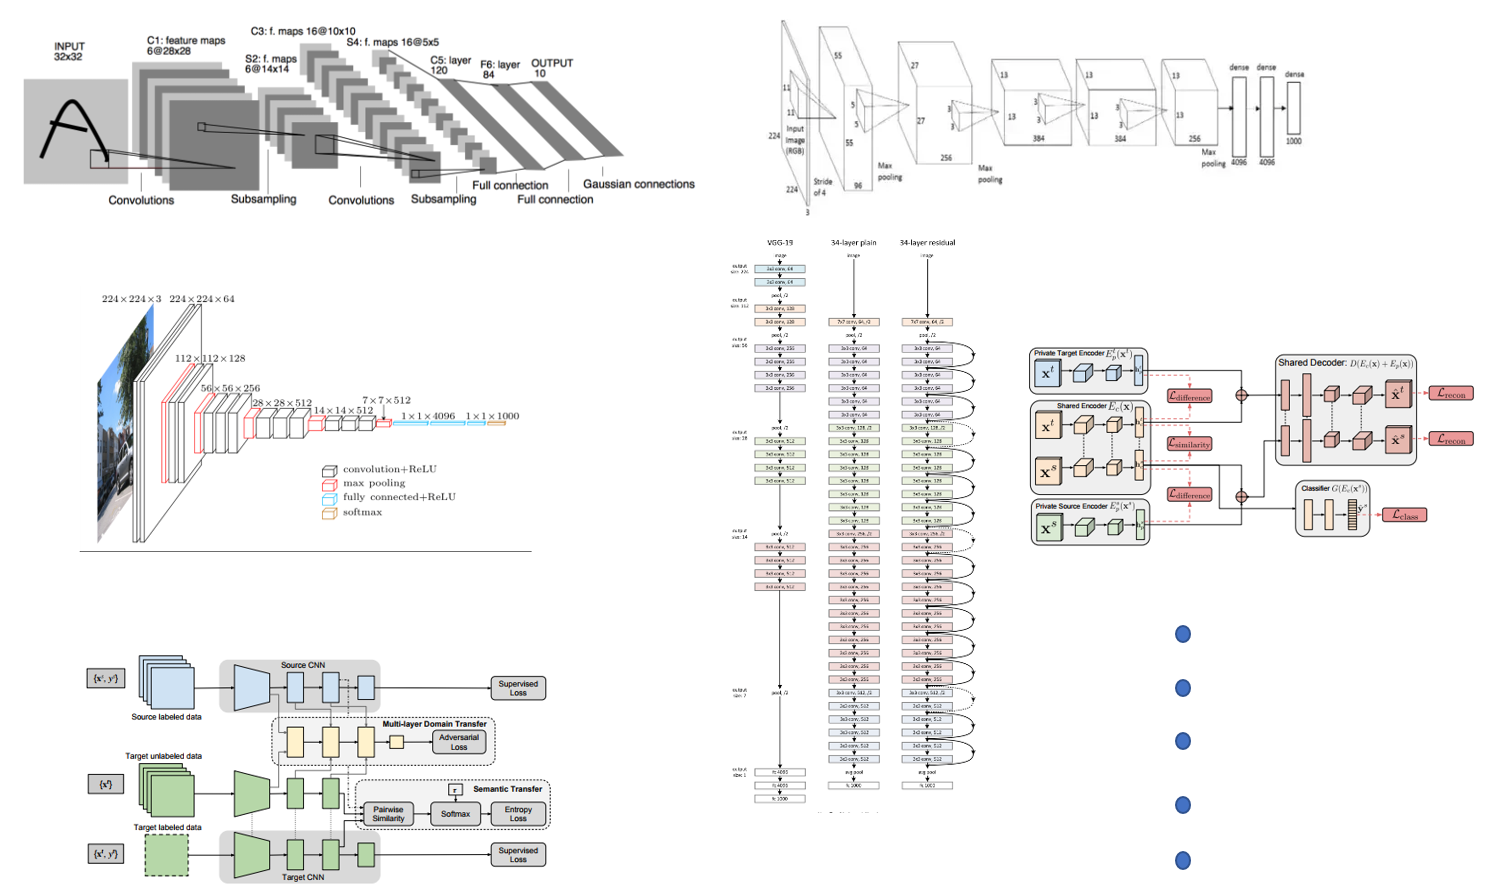
\includegraphics[width=0.8\textwidth]{networks.png}
	}
	\caption{Networks are just special ways to stack all these operations.}
\end{figure}
\end{frame}


\begin{frame}
	\begin{center}
		{\textcolor[rgb]{1 0 0}{\Huge\textsc{Thank you!}}}\bigskip
	\end{center}
\end{frame}




\end{document}
